\documentclass[openany]{book}

\usepackage[DIV=9]{typearea}

\makeatletter
\if@twoside % commands below work only for twoside option of \documentclass
    \newlength{\textblockoffset}
    \setlength{\textblockoffset}{12mm}
    \addtolength{\hoffset}{\textblockoffset}
    \addtolength{\evensidemargin}{-2.0\textblockoffset}
\fi
\makeatother

\usepackage[english]{babel}
\usepackage[utf8]{inputenc} % For spanish characters
\usepackage[T1]{fontenc} % For special characters
\usepackage{times} 
\usepackage{emptypage} 
\usepackage{pgfplots}
\usepackage{graphicx}
\usepackage{color}
\usepackage{float, multirow, rotating}
\usepackage[autolanguage]{numprint}
\usepackage{xspace}
\usepackage{mathtools, amsmath, amsthm, amssymb, enumerate}
\usepackage{hyphenat}
\usepackage{caption, subcaption}
\usepackage{url}
\usepackage{multirow} 
\usepackage{rotating}
\usepackage[ruled, vlined, linesnumbered, resetcount]{algorithm2e}
\usepackage{appendix}
\usepackage{units}
\usepackage{setspace}
\usepackage{fancyhdr}
\usepackage{lipsum}
\usepackage{csquotes}
\usepackage[
  backend=biber,
  style=authoryear,
  citestyle=authoryear,
  backref=true, % include links to pages where the cite is
  mincrossrefs=100000, % Avoid including data of the proceedings
  dashed=minyear, labeldate=true, %Do not group entries from the same authors
  maxbibnames=10, % Use et al for references with more than two names
  maxcitenames=2, % Use et al for references with more than two names
  uniquelist=false, % Use et al for references with more than two names
  firstinits=false, % Use complete names in the bibliography
  natbib=true, % Use natbib
  hyperref=true, % Use hyperref
  isbn=false,doi=false,url=false %Ommit all that info
]{biblatex}

\addto\captionsspanish{}

% Redefine the name of the list of tables
\addto\captionsspanish{
  \renewcommand{\listtablename}{List of Tables}
}

\renewcommand\nameyeardelim{, }
\DeclareNameAlias{sortname}{first-last}
\setlength{\bibitemsep}{\baselineskip}

\newcommand{\image}[4]{
\begin{figure}[!hbtp]
\begin{center}
\includegraphics[scale=#2]{./images/#1}
\caption{#3.}
\label{#4}
\end{center}
\end{figure}
}

\newcommand{\requirement}[3]{
\begin{table}[h!]
\centering
\input{#1}
\caption{#2}
\label{#3}
\end{table}
}

\addto\captionsspanish{\renewcommand{\tablename}{Table}}

\bibliography{references}

\renewcommand{\cite}{\parencite}

\DeclareCiteCommand{\parencite}[\mkbibparens]
  {\usebibmacro{prenote}}
  {\usebibmacro{citeindex}%
    \printtext[bibhyperref]{\usebibmacro{cite}}}
  {\multicitedelim}
  {\usebibmacro{postnote}}

\usepackage{hyperref}
\hypersetup{
   colorlinks,
   linktoc=all, 
   linkcolor=Blue, 
   citecolor=Blue,
   urlcolor=Blue
}

\DefineBibliographyStrings{english}{%
  backrefpage = {page},% originally "cited on page"
  backrefpages = {pages},% originally "cited on pages"
}

\sloppy
\addtocontents{toc}{\protect\thispagestyle{empty}}

% Custom command to add keywords
\newenvironment{keywords}[1]{
  \list{}{\advance\topsep by 0.35cm\relax\small
  \leftmargin=0.7cm
  \labelsep=0.1cm
  \listparindent=0cm
  \itemindent\listparindent
  \rightmargin\leftmargin}\item[\hskip\labelsep\bfseries#1:]}
  {\endlist}

\definecolor{maincolor}{RGB}{240,127,9} 

\pagestyle{plain}
\fancyhf{} % Clears the default header and footer

\fancypagestyle{plain}{
  \fancyhf{}
  \fancyhead{}
  \fancyfoot[RO]{\rule{\textwidth}{0.2pt} \\ \hfill \textbf{\textcolor{maincolor}{COMPUTER SCIENCE DEGREE}}}
  \fancyfoot[LE]{\rule{\textwidth}{0.2pt} \\ \textbf{\textcolor{maincolor}{FINAL DEGREE PROJECT}} | Universidad Francisco de Vitoria \hfill \thepage}
  \renewcommand{\headrulewidth}{0pt}
  \renewcommand{\footrulewidth}{0pt}
}
% Redefine the plain page style for the first page of chapters
\fancypagestyle{fancy}{
  \fancyhf{}
  \fancyhead{}
  \fancyfoot[RO]{\rule{\textwidth}{0.1pt} \\ \hfill \textbf{\textcolor{maincolor}{COMPUTER SCIENCE DEGREE}}}
  \fancyfoot[LE]{\rule{\textwidth}{0.1pt} \\ \textbf{\textcolor{maincolor}{FINAL DEGREE PROJECT}} | Universidad Francisco de Vitoria \hfill \thepage}
  \renewcommand{\headrulewidth}{0pt}
  \renewcommand{\footrulewidth}{0pt}
}


\setcounter{tocdepth}{1}
\newcommand{\myname}{Mois{\'e}s Mart{\'i}nez}
\newcommand{\tutor}{Mois{\'e}s Mart{\'i}nez}
\newcommand{\subject}{Final Degree Project (FDP)}
\newcommand{\mykeywords}{keyword1, keyword2, keyword3, ...}
\newcommand{\mykeywordses}{keyword1, keyword2, keyword3, ...}
\newcommand{\mytitle}{My awesome title}

\hypersetup{pdfauthor={\myname{}},%
            pdftitle={\mytitle{}},%
            pdfsubject={\subject{}},%
            pdfkeywords={\mykeywords{}},%
            pdfproducer={LaTeX},%
            pdfcreator={pdfLaTeX}}

\begin{document}

\renewcommand{\thepage}{\roman{page}}

\pagestyle{empty}

\begin{center}
  
\includegraphics[width=6cm]{./images/logo.jpg}
\end{center}

\vspace{1.25cm}
\begin{center}
{\LARGE UNIVERSIDAD FRANCISCO DE VITORIA}
\end{center}

\vspace{0.15cm}
\begin{center}
{\large \bf  ESCUELA  POLIT{\'E}CNICA SUPERIOR}
\end{center}

\vspace{0.15cm}
\begin{center}
{\large \bf COMPUTER SCIENCE DEGREE}  
\end{center}

\vspace{2.5cm}
\begin{center}
{\Large FINAL DEGREE PROJECT}
\end{center}

\vspace{0.15cm}
\begin{center}
{\Large RESEARCH TRACK}
\end{center}

\vspace{1.0cm}

\begin{center}
  {\LARGE\bfseries\textcolor{maincolor}{\setstretch{1.45}\begin{tabular}{c}
    Autopilot: On-Device AI Desktop\\[0.25em]
    Agent for Hands-Free and Accessible\\[0.25em]
    Windows Automation
  \end{tabular}}}
\end{center}

\vfill
\vspace{0.6cm}

\begin{flushright}
{\normalsize \myname{}}
\end{flushright}

\vspace{0.45cm}
\begin{flushright}
{\normalsize Tutor: \tutor{}}
\end{flushright}


\newpage{}

\phantom{}

\newpage{}

\newcolumntype{P}[1]{>{\centering\arraybackslash}m{#1}}

\begin{center}
    \textbf{CALIFICACI{\'O}N DEL PROYECTO DE FIN DE GRADO}
\end{center}

\vspace{1cm}

\begin{center}
    \begin{tabular}{|P{3cm}|P{9cm}|}
        \hline
        \textbf{CUALITATIVA:\vspace{0.5cm}} & \\ \hline
        \textbf{NUMÉRICA:\vspace{0.5cm}} & \\ \hline
    \end{tabular}
\end{center}

\vspace{1cm}

\begin{center}
    \begin{tabular}{|P{6cm}|P{6cm}|}
        \hline
        \textbf{Conforme Presidente:} & \textbf{Conforme Secretario:} \\ \hline
        & \\[2cm] \hline
        Fdo.: & Fdo.: \\[2cm] \hline
    \end{tabular}
\end{center}

\vspace{1cm}

\begin{center}
    \begin{tabular}{|P{3.8cm}|P{3.8cm}|P{3.8cm}|}
        \hline
        \textbf{Conforme Vocal:} & \textbf{Conforme Vocal:} & \textbf{Conforme Vocal:} \\ \hline
        & & \\[2cm] \hline
        Fdo.: & Fdo.: & Fdo.: \\[2cm] \hline
    \end{tabular}
\end{center}

\vspace{1cm}

\begin{center}
    Lugar y fecha: Pozuelo de Alarcón, a \_\_\_\_ de \_\_\_\_\_\_\_\_\_\_\_\_\_ de 202\_\_
\end{center}

\newpage{}

\pagestyle{empty}

\chapter*{Agradecimientos}

First, I want to thank my supervisor for guiding me through this whole journey. Your support and advice made this project possible, and I'm grateful for all the time you dedicated to helping me grow as a researcher.

To my family, thank you for always being there and believing in me, even during the toughest moments. Your encouragement kept me going.

And to my classmates, thanks for creating that healthy competitive environment that pushed us all to do better. Learning alongside you made this experience way more enjoyable and motivating.
\chapter*{Resumen}

Autopilot es un sistema de automatización de escritorio completamente autónomo para Windows que permite a usuarios con movilidad reducida operar un ordenador utilizando únicamente su voz. El sistema acepta un único comando hablado en lenguaje natural y ejecuta la tarea descrita de principio a fin en el dispositivo local, sin interacción humana adicional, sin conexión a internet y sin que ningún dato abandone el equipo en ningún momento.

El sistema se construye sobre un pipeline neuro-simbólico. Un modelo de reconocimiento de voz transcribe el comando localmente. Un modelo de lenguaje clasifica la intención y extrae los argumentos de la tarea. Un planificador simbólico basado en Fast Downward genera la secuencia de acciones óptima, garantizando un camino de ejecución mínimo y reproducible. Agentes especializados de visión y lenguaje ejecutan cada paso localizando visualmente los elementos de la interfaz en pantalla e interactuando con ellos mediante acciones estándar de ratón y teclado. Un agente final verifica la finalización de la tarea sin revisión humana. Toda la inferencia se ejecuta localmente mediante Ollama con modelos cuantizados a INT4, manteniendo el uso máximo de VRAM por debajo de 8 GB.

El sistema es evaluado sobre siete plantillas de tareas en 21 ejecuciones y comparado con cuatro sistemas alternativos. Autopilot alcanza una tasa de éxito del 100\%, cero errores de planificación y exposición de datos cero, superando a todas las alternativas en autonomía, precisión y privacidad de forma simultánea.

\begin{keywords}{Palabras clave}
  \mykeywordses{}
\end{keywords}

\chapter*{Abstract}

Autopilot is a desktop automation system for Windows that, after receiving a voice command from the user, executes the requested task autonomously end-to-end on the local device. It is designed to enable users with limited motor function to operate a computer through voice interaction without requiring further intervention, internet connectivity, or external data transmission.

This solution has been designed following a neuro-symbolic approach that combines local Deep Neural Networks for language processing and multimodal perception with Automated Planning for reasoning. A local speech recognition model first transcribes the user command, after which a large language model identifies the user intent and extracts the corresponding task parameters. A deterministic planner generates a plan of actions, ensuring deterministic and explainable task execution. Subsequently, some specialised vision-language agents interact with graphical user interface elements through visual grounding and conventional mouse and keyboard inputs. A final verification agent confirms successful task completion without human supervision. All processing and inference are executed locally on the user's device, ensuring complete data privacy and offline operation.

The solution has been evaluated using seven task templates across 21 experimental runs and compared against five alternative desktop automation approaches. Autopilot achieves a 100\% task success rate with zero planning failures and zero data exposure, outperforming all evaluated alternatives in terms of autonomy, execution accuracy, and privacy preservation.
\begin{keywords}{Keywords}
  \mykeywords{}
\end{keywords}


\tableofcontents{}
\listoffigures{}
\listoftables{}
%%\listofalgorithms{}

\pagestyle{fancy}

\cleardoublepage
\setcounter{page}{1}% Start page number with 2
\renewcommand{\thepage}{\arabic{page}}% Arabic numerals for page counter

\chapter{Introduction}
\setcounter{section}{0}

\lipsum[1-2]

% These are some examples of how to cite an article~\cite{nas:1969}, a book~\cite{nas:1972}, and a paper in proceedings~\cite{Keyder:2010}.


\section{Problem description}

\lipsum[1-5]

\section{Outline}

\lipsum[1-5]

\chapter{State of the Art}
\label{chap:state_of_the_art}
\setcounter{section}{0}
\setlength{\parskip}{0.6em}
\section{Symbolic Artificial Intelligence}
\label{sec:symbolic_ai}


Symbolic Artificial Intelligence represents the foundational paradigm that laid the foundations for the field during the mid-20th century until the late 1980s. This deterministic approach is based on \textit{Physical Symbol System Hypothesis}, formulated by Allen Newell and Herbert Simon in 1976 \cite{NewellSimon1976}. This approach aims to represent human knowledge through symbols and states, it represents real world concepts where you can manipulate these using logical rules to solve problems.


Unlike sub-symbolic AI that learns from vast datasets to better understand real world data, symbolic systems are designed from the ground up to tackle only certain domains. Developers have to manually encode rules and constraints related to such domain into a format that the machine understands. This makes the \textit{reasoning process} transparent and interpretable, knowing which actions it took and why, meaning that every decision can be tracked to its origin state, unlike current sub-symbolic AI models where there is an almost unexplainable black box.


Historically, symbolic AI has come has made tremendous breakthroughs such as the \textit{Logic Theorist} (1956), these systems demonstrated that machines could perform expert-level tasks in narrow domains by following a sequence of logical rules. However, they stills faced some key challenges, as seen in the \textit{AI Winter}, handling uncertainty and learning from experience. However the automated planning and the knowledge representation are still at an advantage with the deterministic and long-term planning it offers, against sub-symbolic AI.


In the context of this project, symbolic AI can give a huge advantage over reasoning the series of steps to follow to perform a certain GUI-Actions, from opening an app to sending an email. Making this a deterministic approach, by using PDDL (Planning Domain Definition Language). Therefore the system can generate structured and traceable sequences of actions to navigate graphical interfaces, ensuring that the agent’s behaviour is logical, with a specific goal and deterministic, features which sub-symbolic AI may lack.


{
\interlinepenalty=10000
To achieve this desired behaviour, Symbolic AI relies heavily on Knowledge representation. The most common methodology involves First-Order Logic, which uses predicates and quantifiers to describe the world around us and the relationship between objects, for instance the relationship between a parent and a child folder in order to correctly navigate through them. This architecture was popularized by \textit{Expert Systems}, this established a clear separation between the \textit{Knowledge Base} and the \textit{Inference Engine}, which makes the entire codebase scalable, so there is no need to rewrite the logic every time the knowledge is updated.
\par
}


Within this logical framework, Automated Planning emerged as the specific sub-field dedicated to generating action sequences. The foundation of modern planning is the STRIPS (Stanford Research Institute Problem Solver) system from the early 1970s \cite{FikesNilsson1971}, which introduced the concept of defining actions via preconditions and effects. This means declaring certain conditions that must be true to execute an action, and how the state changes afterward. Mathematically, an action $a$ defines a state transition function $\gamma(s, a)$. If the preconditions are met in the current state $s$ ($Pre(a) \subseteq s$), the new state is computed as:


\begin{equation}
    \gamma(s, a) = (s \setminus Del(a)) \cup Add(a)
\end{equation}


\noindent This implies that the next state is derived by removing the "delete effects" ($Del(a)$) from the current state and adding the "add effects" ($Add(a)$). This logic evolved into the Planning Domain Definition Language (PDDL), which is now the standard research tool for AI planning \cite{McDermott1998}. PDDL allows for a rigorous definition of the domain and problem. Formally, a classical planning task can be defined as the 4-tuple:


\begin{equation}
    \Pi = \langle \mathcal{F}, \mathcal{A}, \mathcal{I}, \mathcal{G} \rangle
\end{equation}


\noindent Where:
\begin{itemize}
    \item $\mathcal{F}$ is a finite set of facts describing the state of the world (e.g. \textit{window\_open}).
    \item $\mathcal{A}$ is a finite set of deterministic actions the agent can perform (e.g. \textit{type\_text}).
    \item $\mathcal{I} \subseteq \mathcal{F}$ represents the Initial State, defining what is true at the start.
    \item $\mathcal{G} \subseteq \mathcal{F}$ represents the Goal State, defining the conditions that must be true to finish.
\end{itemize}

A domain is where you declare the set of actions $\mathcal{A}$, such as clicking, typing, opening an app… Whereas the definition of a problem is where you initialise a set of states and objects and a desired goal. By standardizing these definitions, PDDL enables the creation of agents that can reason about GUI interactions as logical transitions rather than probabilistic guesses. This transition process, where preconditions determine the applicability of actions to transform the system state, is visualized in Figure \ref{fig:pddl_workflow}.
\begin{figure}[H]
    \centering
    % Ajusta el ancho al 80% del texto (puedes cambiar 0.8 por 0.5, 1.0, etc.)
    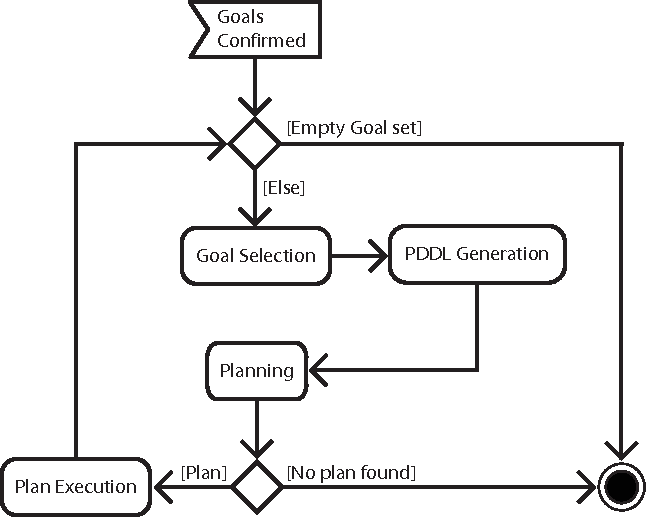
\includegraphics[width=0.5\textwidth]{images/pddl_diagram.png}
    \caption{Workflow of the Planning System.}
    \label{fig:pddl_workflow}
\end{figure}

The PDDL workflow has to start a with goal confirmation, followed by plan generation using search algorithms, such as Breadth First Search, Greedy Best First Search and A*. If a valid plan is found, it proceeds to execution, otherwise, the cycle may restart and choose another path to follow or end without any path found.

However, defining the domain and problem is only the first step, the key challenge is to find the optimal sequence of actions, which requires efficient search algorithms. Classical planning treats the task as a search through a state space, exploring paths from the initial state to the goal. In complex domains like in a GUI interaction system, the state space grows exponentially, this leads to combination of states where an exhaustive search becomes unfeasible. To address this, three main categories of search algorithms are typically considered:


\begin{enumerate}
    \item \textbf{Breadth-First Search (BFS):} This algorithm explores the closer neighbor nodes first, before moving to the next level neighbors. While it guarantees finding the shortest path (optimality), it is computationally expensive as it expands every possible state blindly ($f(n) = g(n)$), making it impractical for large state spaces (complex user tasks).
    
    \item \textbf{Greedy Best-First Search:} This approach prioritizes nodes that appear to be closest to the goal ($f(n) = h(n)$). It is generally faster than BFS it is not optimal. It can find a plan, but it isn’t the most optimal or efficient making it redundant.
    
    \item \textbf{A* (A-Star) Search:} It combines the strengths of the previous two approaches by minimizing a total cost function that balances the actual path cost incurred so far with an intelligent estimate of the remaining cost to the goal \cite{Hart1968}:
    \begin{equation}
        f(n) = g(n) + h(n)
    \end{equation}
    \noindent Where $g(n)$ is the actual cost from the start node to node $n$, and $h(n)$ is the heuristic estimated cost from $n$ to the goal.
\end{enumerate}


To ensure both efficiency and optimality (unnecessary opened apps or clicks), this project relies on A* search. Specifically, it utilizes Fast Downward \cite{Helmert2006}, a state-of-the-art planning system developed by Malte Helmert that has consistently achieved top performance in International Planning Competitions.


Fast Downward is particularly well-suited for this project because of its robust implementation of the LM-cut heuristic (Landmark Cut). This advanced technique analyzes the problem structure to identify \textit{landmarks}, which are facts that must become true at some point in any valid plan to reach the goal. For example, to open a file inside the Documents folder, the system must first navigate to Documents, this navigation is a compulsory landmark.


By calculating the minimum cost of achieving these obligatory intermediate states, LM-cut provides a heuristic that never overestimates the remaining cost. This mathematical property guarantees that Fast Downward finds the optimal plan for the sequence of GUI actions. This optimality is critical as it reduces the number of unnecessary clicks, types and open applications, reducing the surface error area.


Despite these strengths in logical reasoning and planning, Symbolic AI suffers from a critical limitation known as the \textit{Symbol Grounding Problem}. While the planner knows the sequence of actions to execute a task, such as "click the Chrome icon," it has no inherent way to perceive where that icon is located on the screen. It operates on abstract labels, blind to the computer interface. This gap creates a need for Sub-Symbolic AI, which can process unstructured data and bridge this gap between the real world and the logical domain system in PDDL.


\clearpage
\section{Sub-Symbolic Artificial Intelligence}
\label{sec:sub-symbolic_ai}



Sub-Symbolic Artificial Intelligence systems are the next step on machines interacting with the real world. While symbolic AI relies on an explicit declaration of the domain with certain logic rules, objects and goals, Sub-Symbolic AI learn from past experiences (training data) which are representations of the specific domain, so later in a real world test they can behave according to what they saw before. This mimics the human brain, where the model learns from the bottom‑up, extracting patterns from raw data \cite{Rosenblatt1958}.



This is the predominant approach made with Neural Networks, which are computational nodes (neurons) composed of specific layers. This creates a clear distinction between the previous deterministic behaviour mentioned with heuristic algorithms and the creation of relationships which are probabilistic and continuous. Information is not stored in the \textit{Knowledge Base}, but is distributed across the network’s weights that determine the strength of the connection. Therefore, it can generalize from a constructed dataset, understanding ambiguity, noise and incomplete data, where symbolic AI fails to achieve \cite{Rumelhart2002}.



Mathematically, the fundamental unit of these networks, the artificial neuron, processes an input vector $\mathbf{x}$ through a weighted sum and a non-linear activation function $\phi$. This formalizes how the weights modify the output based on the input, allowing the network to learn complex patterns:



\begin{equation}
    \hat{y} = f \left( \sum_{i=1}^{n} (w_n \cdot x_n) + b \right)
\end{equation}


\noindent Where:
\begin{itemize}
    \item $\hat{y}$ is the output (predicted value).
    \item $f()$ is the activation function.
    \item $w_n$ represents the weights.
    \item $x_n$ represents the input features.
    \item $b$ is the bias term.
\end{itemize}



\begin{figure}[H]
    \centering
    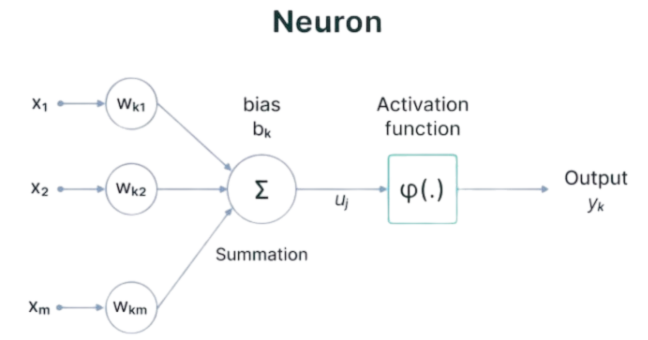
\includegraphics[width=0.5\textwidth]{images/perceptron.png} 
    \caption{An Artificial Neuron where inputs ($x$) are weighted ($w$), summed, and activated to produce an output ($y$).}
    \label{fig:neuron_model}
\end{figure}



However, a single neuron is limited in its capacity to solve complex problems, for instance, it cannot solve non-linear problems like XOR without layers. To address this, neurons are arranged in layers to form a \textit{Multi-Layer Perceptron} (MLP) or Deep Neural Network.



\begin{figure}[H]
    \centering
    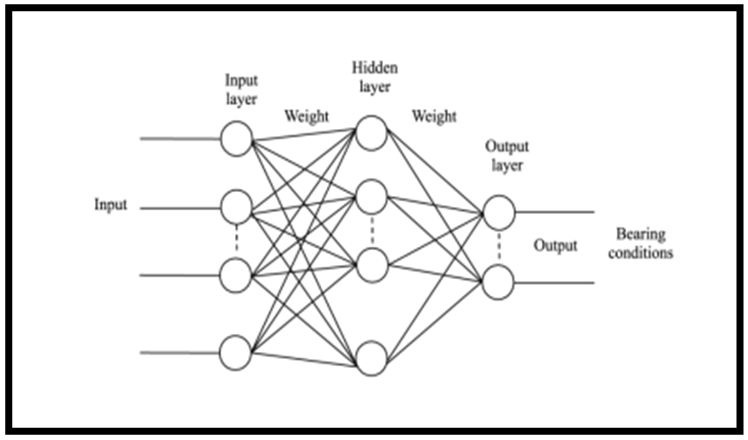
\includegraphics[width=0.5\textwidth]{images/neural_network.jpg} 
    \caption{Architecture of a Deep Neural Network. The system consists of an Input Layer, multiple Hidden Layers for feature extraction, and an Output Layer for final prediction.}
    \label{fig:deep_network}
\end{figure}



This layered architecture is the foundation of the modern models used in this project. Specifically, it enables the use of Large Language Models (LLMs) or Small Language Models (SLMs) for reasoning and Vision-Language Models (VLMs) for perception. These advanced sub-symbolic systems serve as the interface between the user's intent and the symbolic planner, effectively solving the Symbol Grounding Problem described in the previous section. Recent work has explained that symbolic and sub-symbolic methods are not exclusive but can be combined into hybrid architectures that exploit the strengths of both \cite{IlkouKoutraki2020}.

\chapter{Goals}
\setcounter{section}{0}

\section{General Goal}

The general goal of this project is to develop a fully autonomous desktop automation system that enables users with limited mobility to use a Windows computer using only their voice, without requiring any manual intervention in the process.

This system is intended for users affected by conditions such as reduced motor impairment, due to their innability to operate traditional input devices, without learning a new interaction and without selling their data. Existing accessibility tools either demand step-by-step voice commands from the user, shifting the cognitive challenge back to them, or rely on cloud-based services that transmit sensitive data to external servers, where that data is used to train their own models, which may not be acceptable for users with privacy concerns.

This project addresses both limitations by delivering a system that accepts a single natural language voice prompt and executes the described task end-to-end on the local device, with no data leaving the machine at any point. The objective is not to build a faster or more convenient automation tool for technical users, but to ease the path of independent computer use for people who cannot rely on a keyboard and mouse, making any desktop genuinely accessible through natural speech.

\section{List of specific goals}

The following specific goals divide the general objective into concrete, measurable targets. Each goal addresses a distinct requirement that the system must satisfy to be considered a valid accessible automation solution.

\begin{enumerate}

    \item \textbf{Goal 1: Accept voice natural language prompts.} The user must be able to fully describe any task using only a spoken natural language prompt, with no keyboard, mouse, or touch input required from the user at any point. Additionally, the system must not impose a fixed command vocabulary or syntax, meaning it must be a free-form system where the same task can be expressible in different ways and still be correctly understood. This allows the user to interact with the system in a more flexible way, without needing to learn specific commands or phrasing, which is essential for users with cognitive or motor impairments.

    \item \textbf{Goal 2: Make the system fully autonomous.} Once the initial voice prompt has been received, the system must complete the task without any further human input. This autonomy extends beyond simple execution, the system must be capable of detecting when a step has not produced the expected result and act accordingly, without requiring the user to inspect the screen or provide feedback. A system that completes tasks but cannot tell whether it has succeeded is not a reliable accessibility tool.

    \item \textbf{Goal 3: Make the planning layer robust and reproducible.} The planning layer is perhaps the most important component, as it must generate correct, minimal action sequences for every task, with no mistaked, nor any redundancy. Therefore, the same or similar task descriptions must always produce the same correct plan, with no variation across runs. This is not just a quality requirement but a safety requirement, a user who cannot verify the screen or has severe issues to do so must be able to trust that the system always takes the shortest and most predictable path to the goal, without any unexpected detours or mistakes.

    \item \textbf{Goal 4: Achieve a task success rate of 90\%.} It is crucial that the system successfully completes every task it is designed to handle, with no partial executions or unresolved failures, making it precise and reliable.

    \item \textbf{Goal 5: Outperform other local and cloud-based competitors.} The system must not only achieve the highest task success rate among all benchmarked alternatives, both local and cloud-based, but it must do so without any trade-offs, making this system the clear choice on privacy and performance. It must use fewer steps, produce fewer errors, and expose no user data, all at the same time.

    \item \textbf{Goal 6: Complete every task within five minutes on consumer-grade hardware.} Every evaluation run must finish within 300 seconds from the moment the voice prompt is received, running on a standard consumer GPU without any hardware modifications or cloud offloading. A system that is theoretically accessible but takes an impractical amount of time to respond is not usable in practice. The five-minute limit is the threshold above which a user waiting for a result would reasonably abandon the interaction, try to intervene or look for an alternative solution.

    \item \textbf{Goal 7: Run the entire pipeline on local hardware.} The system must operate entirely on the user's own machine, with no external service, remote model, or cloud API involved at any point in the pipeline. All inference must run locally, making the system functional without an internet connection and independent of third-party availability, rate limits, or service outages. This ensures that the system remains usable in any environment, regardless of network access.

    \item \textbf{Goal 8: Guarantee full data privacy with zero data leaving the device.} No user data, including voice recordings, screenshots, task descriptions, file names, or intermediate outputs, are to be transmitted outside the device at any point during execution. The system may manage sensitive data and therefore, it must ensure that all information is stored and processed locally.

    \item \textbf{Goal 9: Interact with the desktop exclusively through standard graphical interface.} The system must operate the computer using only mouse clicks and keyboard on visible graphical elements, the same actions a human user would take. It must never open a terminal  or any other technical interface that would make a non-technical user uncomfortable. A system that solves tasks through the terminal may be functionally correct but minmises the trust of the user, who has no way to understand or verify what the hidden commands are doing.

\end{enumerate}

\section{Validation methods}

Each specific goal is validated through a concrete, measurable method applied during the experimental evaluation described in Chapter~\ref{chap:experiments}.

\begin{enumerate}

    \item \textbf{Goal 1: Accept voice natural language prompts.} All 21 evaluation runs are prompted through a free-form spoken natural language prompt, using Whisper. No keyboard or mouse interaction is performed by the evaluator during task execution.

    \item \textbf{Goal 2: Make the system fully autonomous.} The system organises the execution steps, thanks to Crew AI which helps orchestrate the entire workflow. In the system, the Manager Agent is responsible to orchestrate the entire process, placing each agent in charge of a specific atomic task, and depending on the output of each step to decide the next one. Finally, the Manager Agent, uses the QA Agent for self-verification, which is responsible to check if the task has been completed correctly, without any human feedback, additionally, all runs where evaluated by a human reviewer.
    
    \item \textbf{Goal 3: Make the planning layer robust and reproducible.} Each step across all 21 runs is inspected against the expected PDDL action sequence. Any wrong, missing, or redundant action is counted as a planning error. The validation criterion is \textit{M-04 Planning Error Rate}, which has to be 0. Reproducibility is validated by \textit{M-08 Standard Deviation of Steps}, which has to be 0, confirming that the same template always produces the same number of steps across all three runs.

    \item \textbf{Goal 4: Achieve a task success rate of 90\%.} The system is evaluated over 7 task templates with 3 runs each, for a total of 21 runs. A run is marked successful if the task is completed correctly as confirmed by a human review. The validation criterion is \textit{M-01 Task Success Rate}, which has to be 1 in at least 19 out of 21 runs.

    \item \textbf{Goal 5: Outperform other local and cloud-based competitors.} The system is benchmarked against five alternative systems in a common evaluation table covering all defined metrics. The validation criterion is that the proposed system achieves the best or joint-best value across M-01 TSR, M-04 Planning Error Rate, M-07 Total Error Rate, M-10 Data Exposure Level, and M-11 Total Steps simultaneously, with no metric where it is outperformed by any alternative.

    \item \textbf{Goal 6: Complete every task within five minutes on consumer-grade hardware.} End-to-end latency is measured for each of the 21 runs from the moment the prompt is received to task completion. The validation criterion is \textit{M-03 End-to-End Latency}, which has to be below 300 seconds for every individual run, with no exceptions.

    \item \textbf{Goal 7: Run the entire pipeline on local hardware.} The system is validated by confirming with each run that WiFi and Ethernet connections are disabled, ensuring that no network access is available. Additionally, the system uses all free, local and open-source tools and models.

    \item \textbf{Goal 8: Guarantee full data privacy with zero data leaving the device.} Privacy is validated with each run by ensuring that WiFi and Ethernet connections are disabled, confirming that no data leaves the device, not even after the execution is done. This is reported as \textit{M-10 Data Exposure Level}, where:
        \begin{itemize}
            \item 0: No data leaves the device.
            \item 1: Metadata or task text sent externally.
            \item 2: Sensitive data sent externally.
            \item 3: Sensitive data used to train models.
        \end{itemize}
        The validation criterion is a score of 0.

    \item \textbf{Goal 9: Interact with the desktop exclusively through standard graphical interface.} There is evidence for each run that the system only uses mouse clicks and keyboard inputs on visible graphical elements, with no terminal commands or other technical interfaces involved. This is confirmed by the logs automatically generated, alongside the screenshots taken throughout the process and a final human reviewer.

\end{enumerate}

\chapter{Methodology and Work Plan Overview}
\setcounter{section}{0}

This chapter describes the resources, technical methods, and development methodology that will guide the construction and validation of Autopilot. The constraints that bound the design space are also identified, as they directly shape every architectural decision made throughout the project.

\section{Materials and Resources}

\textbf{Hardware.} The project will be developed and evaluated on an OMEN Gaming Laptop 16 equipped with an AMD Ryzen AI 7 350 processor at 2 GHz, an NVIDIA RTX 5070 Laptop GPU with 8 GB of VRAM, and 32 GB of system RAM, running Windows 11 Home (build 25H2). This machine is representative of the target consumer hardware profile: a mid-range laptop with a discrete GPU capable of running quantised local models without cloud offloading.

\textbf{Models.} Two model families will be used. Gemma4 E4B quantised to INT4 will serve as the Large Language Model, handling intent classification and pipeline orchestration. Qwen3 2B VL quantised to INT4 will serve as the Vision-Language Model, handling screen element detection, pixel coordinate grounding, and task completion verification. Both models will be served exclusively through Ollama and will run entirely on the local GPU. The selection of these models is justified through the benchmarking experiments presented in Chapter~6.

\textbf{Software stack.} The system will be implemented in Python. Ollama will manage all local model inference, loading and unloading each model from VRAM on demand to keep peak memory usage within the hardware constraint. CrewAI will provide the agent orchestration framework, defining each agent's role and handling context passing across pipeline steps. Fast Downward will serve as the PDDL planning engine. The pyautogui library will handle all programmatic mouse and keyboard interactions with the desktop. OpenAI Whisper will perform local speech recognition, avoiding any dependency on cloud-based transcription. LaTeX will be used to produce this report.

\section{Methods}

\textbf{Symbolic planning.} Task planning will be performed using the Planning Domain Definition Language (PDDL). A domain file will define the set of available GUI actions as operators with preconditions and effects; a problem file will specify the initial desktop state and the goal conditions for each supported task. Fast Downward will solve each problem instance using the A* algorithm with the LM-cut heuristic. LM-cut identifies landmarks, facts that must become true in any valid plan, and computes a minimum cost through them, providing an admissible lower bound that guarantees the generated plan is optimal in terms of number of steps.

\textbf{Neural perception.} Screen element detection will be performed by a Vision-Language Model that receives a screenshot and a textual description of a target element and returns a binary YES/NO verdict on whether the element is currently visible. Pixel coordinate grounding will be handled by the same model family in a dedicated role, returning normalised coordinates within a 1000×1000 resolution space that are then mapped to the actual screen resolution. Task completion verification will also rely on the VLM, receiving a final screenshot and confirming whether the goal state has been reached.

\textbf{Natural language understanding and orchestration.} Intent classification will be handled by a local LLM that maps the transcribed voice input to a structured JSON object containing the task template identifier and its required arguments. Pipeline orchestration will also be handled by the same LLM family in a dedicated Manager role, which receives the translated action list and dispatches each specialised agent, branching on agent outputs to handle fallback actions and recovery steps.

\textbf{Model quantisation.} All neural models will be deployed in INT4 precision using post-training quantisation as managed by Ollama. Reducing weight precision from 32-bit float to 4-bit integer cuts memory consumption by approximately 8×, enabling models that would otherwise require more than 20 GB of VRAM to run sequentially within the 7.71 GB available on the target GPU. The accuracy trade-off is verified to be negligible for the instruction-tuned models selected, as confirmed by the model selection benchmarks in Chapter~6.

\textbf{Evaluation protocol.} System performance will be assessed across seven task templates, each executed over three independent runs starting from a clean desktop state with no applications pre-loaded, yielding 21 total evaluation runs. Eleven metrics will be measured across four categories: performance (task success rate, step accuracy, end-to-end latency), reliability (planning error rate, tool hallucination rate, visual hallucination rate, total error rate), consistency (standard deviation of steps and latency), and privacy (data exposure level and total steps). Autopilot will be benchmarked against four alternative systems: Windows Voice Access, Claude Cowork, OpenClaw, and Gemini Computer Use, all evaluated under identical conditions on the same hardware, task templates, and metric set.

\section{Methodology}

The project will follow an iterative and incremental development approach, structured in four sequential phases.

\textbf{Phase 1 — Technology survey and model selection.} The first phase will involve a review of the relevant literature on symbolic planning, large language models, and vision-language models, followed by a practical benchmarking of candidate models for each agent role. Selection will be driven entirely by measured accuracy and resource usage under the hardware constraints of the project, rather than by model size or publication benchmarks.

\textbf{Phase 2 — Pipeline design and implementation.} The neuro-symbolic pipeline will be designed and implemented incrementally, starting from the planning layer and progressively integrating the perception and execution agents. Each agent will be validated in isolation before being connected to the full pipeline. PDDL domain and problem files will be authored for each supported task template and verified against Fast Downward prior to integration.

\textbf{Phase 3 — System evaluation and comparative benchmark.} The complete pipeline will be evaluated over the 21-run protocol described above, and the same evaluation will be applied to each competitor system. Results will be analysed to identify failure modes, architectural trade-offs, and opportunities for post-evaluation improvement.

\textbf{Phase 4 — Report writing and consolidation.} All experimental findings, design decisions, and architectural justifications will be consolidated into this report. Insights from the evaluation may prompt targeted pipeline improvements, which will be incorporated and re-evaluated before the final submission.

\section{Work Plan}

% TODO: Gantt chart to be added here.
% Two Gantt charts are required: the initial plan (drafted at project start) and the final plan
% (reflecting actual completion), with any deviations explained.

\section{Constraints and Limitations}
\label{sec:constraints}

The following constraints are treated as hard boundaries on the system design.

\textbf{VRAM budget.} No more than one model may be resident in GPU memory at any time, and each model must fit within the available VRAM of the target device. This constraint directly drives the choice of quantised models and the sequential loading strategy managed by Ollama.

\textbf{Local-only execution.} No component of the pipeline may invoke an external API or transmit any data over a network connection. All inference, planning, and execution must be performable with no internet access. This is the primary differentiator of the system with respect to cloud-based alternatives and is non-negotiable.

\textbf{Operating system.} The system targets Windows 11 exclusively. All GUI automation relies on the Windows graphical interface, and portability to other operating systems is out of scope.

\textbf{Task template coverage.} The system operates on a predefined set of PDDL task templates. Tasks outside this set cannot be planned by the symbolic layer without authoring a new domain and problem pair.

\textbf{End-to-end latency.} Every task execution must complete within 300 seconds from voice input to verified completion on the target hardware. Runs exceeding this threshold are counted as failures regardless of the desktop state at timeout.

\chapter{Technical Development}
\setcounter{section}{0}

\lipsum[1-4]

\section{System design}

Figure~\ref{fig:class_diagram} shows the class diagram.

\image{class_diagram_example.png}{0.75}{Class diagram example}{fig:class_diagram}

\subsection{Description of functional features}

\lipsum[1-2]

\subsection{Operational Environment}

\lipsum[1-2]

\section{Requirements}
\subsection{Description of requirement attributes}

For the textual description of the different identified requirements, a set of attributes has been selected to describe each requirement. Below is a description of the meaning of each attribute used:

\begin{itemize}
    \item \textbf{Code}: A unique abbreviated identifier for the requirement. It is constructed using the requirement type code followed by a hyphen and three digits. Requirements are divided into functional and non-functional requirements. The codes used are \textbf{FR} for Functional Requirements and \textbf{NFR} for Non-Functional Requirements. For example: \texttt{FR-001}.
    
    \item \textbf{Name}: Extended identification of the requirement.
    
    \item \textbf{Description}: A basic description of the identified requirement.
    
    \item \textbf{Source}: Indicates the source through which the requirement was identified. This value usually corresponds to one or more use case codes.
    
    \item \textbf{Necessity}: Determines the degree of implementation required for the requirement. The possible values are:
    \begin{itemize}
        \item \textbf{Essential}: The requirement must be implemented.
        \item \textbf{Desirable}: It is preferable to implement the requirement, but it is not mandatory.
        \item \textbf{Optional}: The requirement may be implemented, but it is neither important nor mandatory.
    \end{itemize}
    
    \item \textbf{Priority}: Defines the importance of the requirement, allowing the order in which requirements are included in the design and implementation process to be established. The possible values are:
    \begin{itemize}
        \item \textbf{High}: The requirement must be implemented in the early stages of development.
        \item \textbf{Medium}: The requirement should be implemented once high-priority requirements have been completed.
        \item \textbf{Low}: The requirement should be implemented in the final stages of development. These requirements do not affect the correct functioning of the system.
    \end{itemize}
    
    \item \textbf{Stability}: Defines the stability of the requirement throughout the software life cycle. This indicates whether the requirement may be modified during the life cycle. The possible values are:
    \begin{itemize}
        \item \textbf{Stable}: The requirement will not change during the system life cycle.
        \item \textbf{Unstable}: The requirement may change during the system life cycle.
    \end{itemize}
    
    \item \textbf{Verifiability}: Defines the degree to which a requirement can be verified, that is, the extent to which it is possible to confirm that the requirement has been implemented in the developed system. The possible values are:
    \begin{itemize}
        \item \textbf{High}: It is possible to verify that the requirement has been implemented. These requirements usually correspond to core system functionalities.
        \item \textbf{Medium}: It is possible to verify that the requirement has been implemented, but it requires complex testing or inspection of the source code.
        \item \textbf{Low}: It is difficult, or in some cases impossible, to verify whether the requirement has been implemented.
    \end{itemize}
\end{itemize}

\requirement{./tables/requirement_1}{Functional requirement 1}{tab:system_requirement_1}
\chapter{Experiments}
\label{chap:experiments}
\setcounter{section}{0}

\section{Quantitative Evaluation}

All experiments were conducted on the same machine: an OMEN Gaming Laptop 16 with an AMD Ryzen AI 7 350 @ 2 GHz, an NVIDIA RTX 5070 Laptop GPU (7.71 GB VRAM), 32 GB RAM, running Windows 11 Home (25H2) and always plugged in using official charger. Although as it will be seen, this setup over compensates for the need to run these models, using quantization techniques. Cloud-based systems were evaluated over the same Wi-Fi connection to ensure consistent network conditions.


\subsection{Autopilot System Evaluation}

\subsubsection{Model Selection}

Autopilot relies on two different families of models: Vision-Language Models (VLMs), used by the Scout, Vision, and QA agents, and Large Language Models (LLMs), used by the Intention Agent and the Manager Agent. Each family was benchmarked independently, as they present different objectives in the system.

\paragraph{VLM Selection.}
The three VLM roles in Autopilot (Scout, Vision, and QA) share the same underlying model, but they impose different objectives. Scout and QA tasks can be fulfilled using almost any VLM, as most of them are reasonably good with OCR (Optical Character recognition). However, the Vision Agent presents a different challenge, it must return precise screen coordinates. This visual grounding features, is not frequent in VLMs and therefore it was used for the primary selection of the visual model.

Six candidate models were evaluated across three task templates (\textit{Write a Note}, \textit{Search and Open File}, and \textit{Change Text Format in Word}) [ref with each specific prompt or to the bigger table], which all templates require to identify icons and text in screen. The porcentage result for each template, presents with the overall accuracy. Although more models were tested, the INT 4 versions where the most competitive, and therefore the ones presented in the table. The full list of evaluated models is provided in Appendix A.


\begin{table}[H]
\centering
\begin{tabular}{|l|c|c|c|c|c|c|c|}
\hline
\textbf{Model} & \textbf{Params} & \textbf{Quant.} & \textbf{Write} & \textbf{Search} & \textbf{Format} & \textbf{Inference} & \textbf{Avg Vram} \\
 & & & \textbf{(2 steps)} & \textbf{(5 steps)} & \textbf{(5 steps)} & \textbf{Time (s)} & \textbf{(\%)} \\
\hline
Qwen3 2B VL & 2B & INT4 & 100 & 100 & 100 & 34.71 & 32.96 \\
\hline
Qwen3 4B VL & 4B & INT4 & 100 & 100 & 100 & 38.99 & 48.69 \\
\hline
Mistral 3B  & 3B & INT4 & 0   & 0   & 0   & 33.40 & 47.2  \\
\hline
Gemma3 4B   & 4B & INT4 & 0   & 0   & 0   & 31.07 & 51.89 \\
\hline
\end{tabular}
\caption{VLM candidate evaluation across three task templates.}
\label{tab:vlm_candidates}
\end{table}

Both Qwen3 2B VL and Qwen3 4B VL achieved perfect grounding across all three templates, correctly identifying both text and icon targets in every step. Mistral 3B and Gemma3 4B failed entirely at coordinate prediction, hallucinated positions, and were therefore discarded, despite the inference time and the small VRAM used.

Between the two viable candidates, Qwen3 2B VL and Qwen3 4B VL are identical in accuracy (100\% across all templates) but differ in the inference time and the resources used. Since both models achieve the same grounding performance, the smaller model is preferable under the project's consumer hardware constraint. Qwen3 2B VL INT4 was selected as the VLM for all three agent roles (Scout, Vision, and QA).


\paragraph{LLM Selection.}
The LLM must perform two distinct roles: intent classification with the Intention Agent, and task orchestration with the Manager Agent. The model must produce the correct intent name and all required parameters in a structured JSON format, without requiring regular expression fallbacks or post-processing.

The most relevant candidates are summarised in Table~\ref{tab:llm_candidates}; the full list of evaluated models is provided in Appendix A. Each model was tested across two task templates (\textit{Write a Note} and \textit{Change Text Format in Word}).


\begin{table}[H]
\centering
\begin{tabular}{|l|c|c|c|c|c|c|}
\hline
\textbf{Model} & \textbf{Params} & \textbf{Quant.} & \textbf{Write} & \textbf{Format} & \textbf{Inference} & \textbf{Avg} \\
 & & & & & \textbf{Time (s)} & \textbf{Vram (\%)} \\
\hline
Gemma4 E4B         & 4B & INT4  & 100 & 100 & 21.07 & 37.53 \\
\hline
Qwen3 4B Instruct  & 4B & INT4  & 100 & 100 &  2.02 & 25.95 \\
\hline
Qwen3.5 8B         & 8B & INT4  & 100 & 100 &  8.32 & 59.67 \\
\hline
Gemma3 E2B         & 4B & INT 4 & 100 & 100 &  5.29 & 45.56 \\
\hline
Llama3.2 3B        & 3B & INT 4 & 100 & 100 &  2.33 & 17.23 \\
\hline
Ministral3 3B      & 3B & INT 4 & 100 &   0 &  2.26 & 30.90 \\
\hline
\end{tabular}
\caption{LLM candidate evaluation across two task templates.}
\label{tab:llm_candidates}
\end{table}

All six models achieved perfect intent classification on the Write a Note template, and all except Ministral3 3B generalised correctly to a more complex Format Text template. From an entirely Intention Agent perspective, the criteria to select the best model would favour the fastest and most resource-efficient model, which in this case it’s Qwen3 4B Instruct stands out with an inference time of just 2.02 s and 25.95\% average VRAM usage, while Llama3.2 3B offers similar speed at 2.33 s with the lowest VRAM footprint of all candidates (17.23\%).

However, intent classification is only one of the two roles the LLM must fulfil. The same model is also used as the Manager Agent, where it must read the full PDDL plan, maintain execution state across multiple steps, and dispatch each agent Models that performed well as Intention Agents consistently failed as Managers, they lost track of the plan, repeated steps, or didn’t follow the PDDL plan. Of all candidates evaluated, only Gemma4 E4B demonstrated reliable orchestration behaviour across all seven task templates, it’s Effective 4B architecture, gives this model a huge advantage, with far better ability to reason and manage the entire workflow.

\subsubsection{System Evaluation}
\label{sec:autopilot-system-eval}

This section presents the internal performance of the final Autopilot pipeline across all seven task templates, evaluated over 3 runs each (21 total runs). The metrics reported cover the timing breakdown of each pipeline stage, hardware resource utilisation, and the self-reported outcome of the QA Agent. Full per-run details are provided in Appendix A. For all this metrics, Gemma4 E4B to INT 4, was used and as seen in the results, was able to fully manage all workflows, with no errors.

All runs were conducted starting from a clean desktop state, with no applications open and no files pre-loaded in the target directories. This setup was chosen deliberately to maximise the number of steps evaluated per run, ensuring that the pipeline must navigate the full execution path from the initial screen state rather than benefiting from a partially prepared environment. It is important to note that all results presented in this chapter correspond to the system as evaluated at that point, without the initial screen state assessment feature described in Section~\ref{sec:system-design}; that functionality was introduced as a direct consequence of the observations derived from this comparative evaluation.

\paragraph{Manager Evalution}
\begin{table}[H]
\centering
\begin{tabular}{|l|c|c|c|c|c|c|c|}
\hline
\textbf{Template} & \textbf{Intention} & \textbf{Planner} & \textbf{Translator} & \textbf{Scout} & \textbf{Vision} & \textbf{Executor} & \textbf{QA} \\
 & \textbf{(s)} & \textbf{(s)} & \textbf{(s)} & \textbf{(s)} & \textbf{(s)} & \textbf{(s)} & \textbf{(s)} \\
\hline
Write a Note      & 11.43 &  2.61 & 1.89 &  6.36 & N/A  &  7.02 & 1.05 \\
\hline
Create Doc/Folder &  7.82 &  2.10 & 0.55 &  2.57 & 1.58 &  9.45 & 0.61 \\
\hline
Search \& Open   & 13.59 &  1.46 & 1.01 &  1.81 & 2.61 & 16.28 & 1.11 \\
\hline
Search Text       & 10.85 &  1.98 & 1.88 &  3.86 & 3.81 & 19.27 & 3.36 \\
\hline
Delete Text       & 11.94 &  1.47 & 1.69 &  8.20 & 5.01 & 27.66 & 1.08 \\
\hline
Format Text       & 15.15 &  1.38 & 3.28 &  7.43 & 4.64 & 19.25 & 3.39 \\
\hline
Copy and Paste    &  8.97 &  1.97 & 2.45 &  6.05 & 1.66 & 16.11 & 2.42 \\
\hline
Global            & 11.39 &  1.85 & 1.82 &  5.18 & 3.22 & 16.43 & 1.86 \\
\hline
\end{tabular}
\caption{Autopilot average Manager Thinking timings (seconds) per task template, averaged across 3 runs each.}
\label{tab:manager_timings}
\end{table}

Across all templates, intent classification is the main cost, averaging 11.39 s globally. This is expected, as it is the first initialization of the model and might take more time to power up and load to the VRAM. Afterwards, the model is already loaded and call the Planner Agent quickly, the same thing happens for the translator agent that is called efficiently right after the PDDL planning.

The Scout Agent time varies from nearly 2s up to almost 8s, this is due the numerous calls during more complex tasks, such as formatting a specific text in Word. Moreover, the Vision Agent is more direct, due to the straight and more natural approach. The execute action, has the highest time, this is because the Manager Agent, must think thoroughly, what the response for the Scout and Vision Agent was, and therefore give the executor the correct parameters for the given the specific situation, to execute a fallback action, a click, type or find a specific text.

Finally, the QA Agent, is always the last step of the workflow, therefore due to the explicit declaration in the prompt, the manager agent can do this step very quickly and precise.

\paragraph{Agents Evaluation}
\begin{table}[H]
\centering
\begin{tabular}{|l|c|c|c|c|c|c|c|}
\hline
\textbf{Template} & \textbf{Intention} & \textbf{Planner} & \textbf{Translator} & \textbf{Scout} & \textbf{Vision} & \textbf{Executor} & \textbf{QA} \\
 & \textbf{(s)} & \textbf{(s)} & \textbf{(s)} & \textbf{(s)} & \textbf{(s)} & \textbf{(s)} & \textbf{(s)} \\
\hline
Write a Note      & 20.41 & 0.45 &    0 & 2.39 & N/A  &  7.51 & 4.17 \\
\hline
Create Doc/Folder & 18.49 & 0.19 &    0 & 1.38 & 1.34 & 11.30 & 3.36 \\
\hline
Search \& Open   & 22.98 & 0.58 &    0 & 2.38 & 3.74 & 12.90 & 3.63 \\
\hline
Search Text       & 21.79 & 0.43 &    0 & 2.36 & 2.03 & 13.22 & 3.91 \\
\hline
Delete Text       & 25.63 & 0.47 &    0 & 2.11 & 2.04 & 15.86 & 4.58 \\
\hline
Format Text       & 31.17 & 0.45 & 0.01 & 7.43 & 4.64 & 19.66 & 4.09 \\
\hline
Copy and Paste    & 23.28 & 0.44 &    0 & 2.08 & 1.91 & 12.32 & 4.04 \\
\hline
Global            & 23.29 & 0.42 &    0 & 2.87 & 2.63 & 13.26 & 3.97 \\
\hline
\end{tabular}
\caption{Autopilot average Agent times (seconds) per task template averaged across 3 runs each.}
\label{tab:agent_timings}
\end{table}

This table breaks down the average execution time per agent across all seven templates. The Intention agent dominates the pipeline, accounting for 23.29 s globally, which represents over half of the total end-to-end time in most templates. This is expected given that it runs a quantized 4B language model locally to parse all 7 templates, from free form speech into a structured JSON. Moreover, the Intention Agent is the first step of the pipeline, therefore it might take more time to power up and load to the VRAM, which can explain the higher time compared to the rest of the agents

The next agent in line is the Planner, whichis consistently negligible at 0.42 s globally, reflecting the deterministic and lightweight nature of Fast Downward. The Translator is effectively zero across all templates, due to its pure code operation with no model inference.

Scout Agent averages 2.87 s globally, with Format Text being the highest at 7.43 s due to the greater number of visibility checks required when locating text or UI elements. Vision is N/A for Write a Note, the only template where no coordinate grounding is needed, this task only requires opening Notepad and typing. Across the remaining templates, Vision averages 2.63 s, remaining stable and predictable, due to the straightforward prompt and task it has to complete. 

Then, the Executor Agent is the second most expensive agent at 13.26 s globally, this time is static, as the system has to wait until the Windows system has updated its state, otherwise, there is a risk of capturing incorrect screenshots, or typing/clicking when the OS isn't ready yet. Finally, QA is stable across all templates at around 3.97 s globally, consistent with its fixed role and custom prompt, which is designed to be concise and direct to the point, making it easier for the model to understand and answer quickly.

\paragraph{Resources Evaluation}

\begin{table}[H]
\centering
\begin{tabular}{|l|c|c|c|c|}
\hline
\textbf{Template} & \textbf{CPU avg} & \textbf{RAM avg} & \textbf{GPU Util.} & \textbf{GPU Mem.} \\
 & \textbf{(\%)} & \textbf{(\%)} & \textbf{avg (\%)} & \textbf{avg (\%)} \\
\hline
Write a Note      & 25.3 & 70.2 & 20.9 & 81.0 \\
\hline
Create Doc/Folder & 18.6 & 78.0 & 33.0 & 80.0 \\
\hline
Search \& Open   & 25.9 & 71.4 & 23.9 & 74.1 \\
\hline
Search Text       & 25.9 & 74.1 & 22.6 & 78.8 \\
\hline
Delete Text       & 26.6 & 70.4 & 22.4 & 81.0 \\
\hline
Format Text       & 25.7 & 69.4 & 21.3 & 74.6 \\
\hline
Copy \& Paste    & 25.2 & 69.9 & 22.7 & 81.0 \\
\hline
Global            & 24.7 & 71.9 & 23.8 & 78.6 \\
\hline
\end{tabular}
\caption{Autopilot average resource usage per task template, averaged across 3 runs.}
\label{tab:resource_usage}
\end{table}

The regarding resource usage is a key aspect in this system, due to the complex organisation of the agents, it is important to reduce the resource consumption. We can see how GPU memory averages between 74\% and 81\% across templates, consistent with Ollama's managed memory, the quantized models are loaded into VRAM on demand and remain resident until unloaded, causing memory usage to stay elevated throughout execution. GPU utilisation averages between 21\% and 33\% and dropping to near zero between agent calls. CPU usage remains modest at around 25\% on average, and RAM usage stays stable between 70\% and 78\%, confirming that the system operates comfortably within consumer hardware constraints.

Finally, it is important to note, that the QA Agent reported success (YES) in 86\% of runs globally (18 out of 21). The two \textit{NO} responses occurred during the \textit{Format Text} template, where the QA Agent incorrectly judged the formatting task as incomplete despite human verification confirming success. Despite altering the prompt several times to be more concise and even telling the model to compare the final text with other non-formatted text. Meaning that the QA Agent's screenshot, despite being in high-quality, Qwen3 only process images in 1000x1000, therefore the image distortion, not only in quality but in the aspect ratio, can lead the QA Agent to be less precise.

\subsection{Comparative Evaluation}

This section presents a comparative benchmark of Autopilot against five alternative desktop automation systems. All systems were evaluated on the same seven task templates, over 3 runs each, on the same hardware described in Section 1.1. Steps across all systems are normalised to Autopilot's PDDL action schema, one step corresponds to one atomic PDDL action. This normalisation was possible because Gemini CU and Gemini CU Screenshot produce execution logs, Claude Cowork exposes a visible thought process, allowing each system's actions to be mapped to the equivalent PDDL actions and Windows Voice Access uses direct user's commands that can easily be mapped to the same schema, although there are audio recordings to verify the exact commands used.

\subsubsection{Competitor Systems}

\paragraph{Windows Voice Access}
Windows Voice Access is a built-in accessibility feature in Windows 11 that allows users to control their computer using voice commands. It provides up to 80 commands for various actions, such as opening applications, clicking buttons and typing, which are the core actions required to complete the task templates. The system was tested with the laptop's built-in microphone, and the command execution was verified through audio recordings to ensure that the correct commands were issued for each step in the task templates. Here the main disadvantage of this system is that the user is the planner and WVA is the executor, meaning that the user cannot give full prompt at the beginning of the task, but must give commands step by step, which fails to meet the requirement of a single prompt and fully autonomous execution. Moreover, the user must be familiar with the specific commands and their syntax, which can be a barrier for non-technical users.

\paragraph{Claude Cowork}
Claude Cowork is a collaborative cloud based AI system developed by Anthropic, designed to assist users in various tasks through natural language interactions. One of it's functionalities (still in Beta) is computer use. It allows the user to give a single prompt describing the task they want to accomplish, and then the system takes care of executing it, using the GUI, terminal or any available tool. The system provides a visible thought process, where it explains the steps it is taking to complete the task, which allows for a detailed evaluation of its performance and the reasoning behind its actions. 

Claude Cowork's main objective is to serve as an accessible alternative to Claude Code for non-technical users, providing a dedicated Windows application with a more intuitive interface. However, during computer use sessions, the system uses other tools, such as opening the terminal or calling the Windows Run dialog (Win+R), actions that despite being effective, they may generate distrust in users who are not familiar.

Unlike Autopilot's PDDL architecture, Claude Cowork operates reactively, meaning that it captures a screenshot, decides an action, executes it, and repeats the cycle until the goal is completed, with no first planning stage. This approach is great for simple tasks, which are very straightforward and don't require any long and complex reasoning, however, as evidenced in the recorded runs and later reflected in the comparative metrics, it also leads to non-optimal execution paths in more complex tasks, where the system becomes repetitive after reaching dead ends or fails to identify the most direct route to the objective. 

A recurring pattern observed across templates is that Claude Cowork opens a target file or window and immediately minimises it, as documented in Run 3 of the \textit{Search \& Open} template, meaning that in the next step, Claude thinks the task was not completed, despite being completed. Although, the system's fast actions allow it to recover and complete most tasks within a competitive time.

\paragraph{OpenClaw}
OpenClaw is an open-source desktop automation system designed for the model to use various tools at hand to comply with user demands, without providing a dedicated GUI. It was evaluated using Gemma4 E4B INT4 and Qwen3.5 8B INT4 across two tool integration approaches: skills and MCPs, tested independently.

Two skills were evaluated: Desktop Control [ref], which covers mouse, keyboard, screen capture, and clipboard management via OpenCV, and Windows UI Automation [ref], which automates Windows GUI interactions through native APIs and PowerShell. Two MCPs were also tested: PyAutoGUI MCP [ref], which exposes mouse, keyboard, and screen control as model-callable tools, and Windows-MCP by CursorTouch [ref], which combines PyAutoGUI with the Windows UIAutomation framework for native element interaction without computer vision. None of these configurations was sufficient for the model to reliably plan and execute the task templates.

\paragraph{Gemini Computer Use}
Gemini Computer Use (Gemini CU) is a cloud-based desktop automation system developed by Google, that allows users to control the desktop through natural language commands. However, it currently only offers an API with no dedicated user interface, which makes it less accessible for non-technical users. Thus, a Python script had to be developed in order to interact with the model. Both variants used \textit{gemini-3-flash-preview} as the underlying model.

Two variants were implemented and evaluated, due to the specific recommendation in the Google documentation, which states it is better for the developer to provide a screenshot after each action, rather than leaving the model to decide when to capture the screen. Although, this goes against the core principle of fully autonomous execution, therefore, both approaches were implemented and evaluated to determine the best integration pattern for this system.

In the first variant, Gemini CU, \textit{take\_screenshot} is exposed as one of the available tools, the model decides autonomously when to observe the screen, calling it only when it deems necessary. In the second variant, Gemini Screenshot (Gemini SS), the screenshot tool is removed entirely and the orchestration script automatically captures and injects a screenshot into the conversation after every action, ensuring the model always has an up-to-date view of the desktop state before its next decision.

A significant practical limitation observed throughout both evaluations was API availability. Out of 42 total runs, 22 had to be repeated due to the API returning resource exhaustion errors, indicating that the service was under heavy load. This instability introduces a substantial reliability concern for any deployment that depends on consistent response times.


\subsubsection{Evaluation Metrics}

Eleven metrics were defined across four categories: performance, reliability, variability, and privacy. Table~\ref{tab:metrics} summarises each metric, its description, and its possible values or range.

\begin{table}[H]
\centering
\small
\begin{tabular}{|l|p{3.5cm}|p{5cm}|p{3cm}|}
\hline
\textbf{ID} & \textbf{Name} & \textbf{Description} & \textbf{Values / Range} \\
\hline
M-01 & Task Success Rate (TSR) & Average proportion of runs completed successfully & 0 to 1 \\
\hline
M-02 & Step Accuracy & Fraction of executed steps that were error-free & 0 to 1 \\
\hline
M-03 & End-to-End Latency & Average time from prompt to completion, if time exceed 5 minutes the task is aborted. & seconds \\
\hline
M-04 & Planning Error Rate & Fraction of steps with wrong or missing actions & 0 to 1 \\
\hline
M-05 & Tool Hallucination Rate & Fraction of steps invoking a non-existent or incorrect tool & 0 to 1 \\
\hline
M-06 & Visual Hallucination Rate & Fraction of steps where the vision model misidentified on-screen elements & 0 to 1 \\
\hline
M-07 & Total Error Rate & Combined error rate (sum of M-04, M-05, M-06) & 0 to 1 \\
\hline
M-08 & Standard Deviation of Steps & Variability of step count across repetitions, the higher the deviation, the less consistent & Float \\
\hline
M-09 & Standard Deviation of Latency & Variability of latency across repetitions, the higher the deviation the less consistent & Float \\
\hline
M-10 & Data Exposure Level & Amount of sensitive data sent outside the device & 
      \begin{tabular}[c]{@{}l@{}}
        0: No data leaves the device \\
        1: Metadata or task text sent externally \\
        2: Sensitive data sent externally \\
        3: Sensitive data used to train models \\
      \end{tabular} \\
\hline
M-11 & Total Steps & Total number of steps taken to complete a run & integer \\
\hline
\end{tabular}
\caption{Evaluation metrics used in the comparative benchmark.}
\label{tab:metrics}
\end{table}

\subsubsection{Full System Comparison}

Table~\ref{tab:full_comparative} presents all six systems evaluated across the same seven task templates with three runs each, providing an unconstrained baseline before any filtering is applied.

\begin{table}[H]
\centering
\begin{tabular}{|p{4.5cm}|c|c|c|c|c|c|}
\hline
\textbf{Metric} & \textbf{Autopilot} & \textbf{WVA} & \textbf{OpenClaw} & \textbf{Claude} & \textbf{Gemini} & \textbf{Gemini} \\
 & & & & \textbf{CW} & \textbf{CU} & \textbf{SS} \\
\hline
M-01 Task Success Rate (TSR)        & 1.000  & 1.000 & 0.000 & 1.000 & 0.333 & 0.952 \\
\hline
M-02 Step Accuracy                  & 0.925  & 0.968 & 0.000 & 0.775 & 0.479 & 0.893 \\
\hline
M-03 End-to-End Latency             & 111.83 & 47.00 & - & 111.75 & 47.90 & 77.67 \\
\hline
M-04 Planning Error Rate            & 0.000  & 0.000 & 0.000 & 0.225 & 0.358 & 0.107 \\
\hline
M-05 Tool Hallucination Rate        & 0.000  & 0.000 & 0.000 & 0.000 & 0.163 & 0.000 \\
\hline
M-06 Visual Hallucination Rate      & 0.075  & 0.032 & 0.000 & 0.000 & 0.000 & 0.000 \\
\hline
M-07 Total Error Rate               & 0.075  & 0.032 & 0.000 & 0.225 & 0.521 & 0.107 \\
\hline
M-08 Standard Deviation of Steps    & 0.000  & 0.034 & 0.000 & 0.139 & 0.588 & 0.191 \\
\hline
M-09 Standard Deviation of Latency  & 0.123  & 0.095 & 0.000 & 0.152 & 0.556 & 0.527 \\
\hline
M-10 Data Exposure Level            & 0      & 0     & 0     & 3     & 3     & 3     \\
\hline
M-11 Total Steps                    & 4.57   & 10.90 & 0.000 & 6.38  & 8.48  & 5.86  \\
\hline
\end{tabular}
\caption{Full comparative evaluation across all six systems with three runs per template.}
\label{tab:full_comparative}
\end{table}

A cross-cutting observation that emerged from reviewing all competitor systems is that none of them performs an initial assessment of the current desktop state before committing to a plan or action. Every system evaluated, whether reactive like Claude CW and Gemini CU or command-driven like WVA, assumes a blank slate and begins issuing actions immediately, without first checking what is already visible on screen. This means they cannot take advantage of elements that are already open, nor detect early that the required conditions are not yet met. After analysing these results, it was decided to extend Autopilot with an initial screen state check: before invoking the Planning Agent, the Manager Agent now calls the Scout Agent to assess what is currently visible on the desktop, allowing the pipeline to ground its plan in the actual context from the very first step. This feature was not present during the experiments reported in this chapter and is therefore not reflected in the metrics above; it represents a direct improvement derived from the comparative analysis.

This section focuses on WVA and Gemini SS, the two systems excluded from the next comparison, and how they relate to Autopilot. The remaining systems (OpenClaw, Claude CW, and Gemini CU) are discussed in the following sections.

WVA achieves a perfect TSR (1.000) and actually outperforms Autopilot on step accuracy (0.968 vs 0.925) and total error rate (0.032 vs 0.075), with a lower latency of 47.00 s. However, these numbers come at the cost of autonomy: WVA requires the user to issue commands step by step, which is why it needs 10.90 steps on average, more than double Autopilot's 4.57. It is not a fair autonomous competitor, but it serves as a bottom line of current alternatives to assistive technologies. Moreover, WVA has as default settings to mantain everything locally with no data being sent across servers although this feature can be turned on at any time.

Gemini SS scores TSR 0.952 and a total error rate of 0.107, making it the second most accurate system. The constant scrennshot feedback injected after each action clearly helps the model keep track of its progress and future actions, resulting in lower planning errors (0.107) and no tool or visual hallucinations. Despite this, Gemini SS is excluded from the later autonomous comparison because the screenshot injection is managed externally by the orchestration script, not by the model itself, which breaks the core requirement of fully autonomous execution. Additionally, Gemini SS sends information to external servers, where they use this data to better train the models.

\subsubsection{Autonomous Systems}

Table~\ref{tab:autonomous_comparative} restricts the comparison to systems that run fully autonomously, excluding WVA and Gemini SS for reason mentioned before. Therefore, we can directly compare the core autonomous capabilities of Autopilot, OpenClaw, Claude CW, and Gemini CU.

\begin{table}[H]
\centering
\begin{tabular}{|p{4.5cm}|c|c|c|c|}
\hline
\textbf{Metric} & \textbf{Autopilot} & \textbf{OpenClaw} & \textbf{Claude} & \textbf{Gemini} \\
 & & & \textbf{CW} & \textbf{CU} \\
\hline
M-01 Task Success Rate (TSR)        & 1.000  & 0.000 & 1.000 & 0.333 \\
\hline
M-02 Step Accuracy                  & 0.925  & 0.000 & 0.775 & 0.479 \\
\hline
M-03 End-to-End Latency             & 111.83 & - & 111.75 & 47.90 \\
\hline
M-04 Planning Error Rate            & 0.000  & 0.000 & 0.225 & 0.358 \\
\hline
M-05 Tool Hallucination Rate        & 0.000  & 0.000 & 0.000 & 0.163 \\
\hline
M-06 Visual Hallucination Rate      & 0.075  & 0.000 & 0.000 & 0.000 \\
\hline
M-07 Total Error Rate               & 0.075  & 0.000 & 0.225 & 0.521 \\
\hline
M-08 Standard Deviation of Steps    & 0.000  & 0.000 & 0.139 & 0.588 \\
\hline
M-09 Standard Deviation of Latency  & 0.123  & 0.000 & 0.152 & 0.556 \\
\hline
M-10 Data Exposure Level            & 0      & 0     & 3     & 3     \\
\hline
M-11 Total Steps                    & 4.57   & 0.000 & 6.38  & 8.48  \\
\hline
\end{tabular}
\caption{Autonomous systems comparison: Autopilot, OpenClaw, Claude CW, and Gemini CU.}
\label{tab:autonomous_comparative}
\end{table}

This section focuses on Claude CW and Gemini CU, the two systems excluded from the final comparison, and how they relate to Autopilot. OpenClaw is also present but fails entirely (TSR 0.000), and is discussed in depth in the following section alongside Autopilot.

Claude CW matches Autopilot on TSR (1.000) but accumulates a planning error rate of 0.225, compared to Autopilot's zero, which is consistent with its reactive architecture: no upfront plan means the model occasionally chooses the wrong action or gets stuck. This also translates into more steps on average (6.38 vs 4.57) and a higher step standard deviation (0.139 vs 0.000). On the positive side, Claude CW produces no tool or visual hallucinations, meaning its errors are purely reasoning-based rather than perceptual. However, as a cloud system, it transmits screenshots and conversation context on every action (M-10 = 3), which rules it out for privacy-sensitive deployments.

Gemini CU performs significantly worse, achieving only TSR 0.333 and accumulating errors across all three categories: planning (0.358), tool hallucination (0.163), and a total error rate of 0.521. It is also the least consistent system, with a step standard deviation of 0.588 and a latency standard deviation of 0.556. Like Claude CW, it carries a data exposure level of 3. Both cloud systems are excluded from the final comparison for these reasons. The next section isolates Autopilot and OpenClaw as the only two fully local candidates.

\subsubsection{Fully Local Systems}

Table~\ref{tab:local_comparative} isolates the two systems that run entirely on local hardware without any cloud dependency, enabling a direct comparison of on-device automation performance.

\begin{table}[H]
\centering
\begin{tabular}{|p{4.5cm}|c|c|}
\hline
\textbf{Metric} & \textbf{Autopilot} & \textbf{OpenClaw} \\
\hline
M-01 Task Success Rate (TSR)        & 1.000  & 0.000 \\
\hline
M-02 Step Accuracy                  & 0.925  & 0.000 \\
\hline
M-03 End-to-End Latency             & 111.83 & - \\
\hline
M-04 Planning Error Rate            & 0.000  & 0.000 \\
\hline
M-05 Tool Hallucination Rate        & 0.000  & 0.000 \\
\hline
M-06 Visual Hallucination Rate      & 0.075  & 0.000 \\
\hline
M-07 Total Error Rate               & 0.075  & 0.000 \\
\hline
M-08 Standard Deviation of Steps    & 0.000  & 0.000 \\
\hline
M-09 Standard Deviation of Latency  & 0.123  & 0.000 \\
\hline
M-10 Data Exposure Level            & 0      & 0     \\
\hline
M-11 Total Steps                    & 4.57   & 0.000 \\
\hline
\end{tabular}
\caption{Fully local systems comparison: Autopilot and OpenClaw.}
\label{tab:local_comparative}
\end{table}

The fully local comparison yields the starkest result in the entire benchmark: Autopilot completes every task (TSR 1.000) while OpenClaw completes none (TSR 0.000). Both systems run on the same hardware, use comparable quantised models, and share a data exposure score of zero, so the gap cannot be attributed to hardware, cloud access, or privacy trade-offs.

The difference is purely architectural. Autopilot separates intention parsing, symbolic planning, visual grounding, and execution into specialised agents, each with a focused role and a tailored prompt. OpenClaw relies on a single general-purpose LLM to reason about the full task, decide which tool to invoke, and recover from failures, all in one unstructured loop. None of the tool configurations tested, whether skills or MCPs, were sufficient to overcome this limitation. The results show that access to the right tools is not enough without a planning layer that structures how they are used.

This directly supports one of the central claims of this project: running local models is necessary for privacy and offline operation, but it is not sufficient for reliable automation. The structured pipeline is the critical component, and Autopilot demonstrates that strong performance on consumer hardware is achievable without any cloud dependency.

\section{Qualitative Evaluation}

In addition to the quantitative benchmark, a qualitative user study was conducted to assess real-world perceived usability and accessibility. Ten participants were invited to interact with Autopilot on the same hardware used for the comparative evaluation described in Section~\ref{sec:autopilot-system-eval}. Each participant issued a free-form voice command of their choice, covering six of the seven supported task templates, and then completed a Google Forms survey of six Likert-scale questions (1 = worst, 5 = best) alongside an optional free-text comment. All ten participants confirmed that the system completed their requested task successfully.

Table~\ref{tab:qualitative_responses} reports the individual responses of each participant. Column headers are abbreviated; their full descriptions are: \textit{Recovery} (ability to recover from errors), \textit{Behaviour} (absence of detours or unexpected actions), \textit{Privacy} (perceived importance of local processing), \textit{Accessibility} (suitability for users with motor difficulties), \textit{Daily Use} (likelihood of daily use), and \textit{vs Others} (likelihood of choosing Autopilot over other alternatives).

\begin{table}[H]
\centering
\begin{tabular}{|c|l|c|c|c|c|c|c|}
\hline
\textbf{\#} & \textbf{Task} & \textbf{Recovery} & \textbf{Behaviour} & \textbf{Privacy} & \textbf{Accessibility} & \textbf{Daily Use} & \textbf{vs Others} \\
\hline
1  & Open File      & 5 & 2 & 4 & 4 & 4 & 4 \\
\hline
2  & Format Text    & 4 & 2 & 5 & 5 & 3 & 3 \\
\hline
3  & Format Text    & 3 & 4 & 2 & 2 & 2 & 4 \\
\hline
4  & Open File      & 5 & 5 & 5 & 5 & 4 & 4 \\
\hline
5  & Copy \& Paste  & 5 & 4 & 2 & 4 & 4 & 3 \\
\hline
6  & Create Folder  & 4 & 5 & 5 & 4 & 4 & 3 \\
\hline
7  & Write Note     & 5 & 5 & 4 & 4 & 4 & 4 \\
\hline
8  & Search Text    & 4 & 4 & 4 & 4 & 3 & 4 \\
\hline
9  & Write Note     & 5 & 4 & 4 & 5 & 5 & 4 \\
\hline
10 & Copy \& Paste  & 5 & 5 & 5 & 4 & 5 & 3 \\
\hline
\textbf{Mean} & & \textbf{4.5} & \textbf{4.0} & \textbf{4.0} & \textbf{4.1} & \textbf{3.8} & \textbf{3.6} \\
\hline
\end{tabular}
\caption{Qualitative user study responses. All ratings on a 1--5 scale (1 = worst, 5 = best).}
\label{tab:qualitative_responses}
\end{table}

Error recovery received the highest mean score (4.5), indicating that participants consistently perceived the system as capable of handling mistakes without failing the task. One participant noted: \textit{Very impressive how despite identifying wrong certain elements in the screen it detects that and is able to continue to next step.} Behavioural predictability averaged 4.0, the two lower scores (both 2) corresponded to participants who attempted the Format Text template, where a higher number of intermediate steps and the visual grounding behaviour may have appeared less direct to a first-time user. Privacy scored 4.0 on average, though opinions were notably different, with participants of a more technical background rating it highest, while one noted \textit{``it is not very important to me the data in my device''}, reflecting that the perceived value of local processing depends on the user. Accessibility suitability for motor impaired people averaged 4.1, with one outlier (score 2) corresponding to the same participant who reported transcription errors.

Likelihood of daily use (3.8) and preference over alternatives (3.6) were the lowest scoring dimensions, consistent with the system's current limitation to seven task templates and the latency due to the complex orquestration in local INT4 inference. Two participants specifically mentioned execution time, with one commenting \textit{``It took a while, it wasn't quick.''} Speech recognition accuracy was the most frequently cited area for improvement, two participants noted that the system did not transcribe their command correctly on the first attempt, although in both cases the task was completed successfully.

\chapter{Ethical Implications and Social Impact}
\setcounter{section}{0}
\setlength{\parindent}{0pt}
\section{AI-Based Systems Ethical Impact}

The rapid advancements in artificial intelligence systems have raised a new debate
on its ethical implications. Traditionally, software programs execute explicit and
deterministic instruction, which are given and controlled by a human. Also, the same
input always gave the same output, but if a misbehaviour occurred, one could always
traceback to a specific block of code. However, agentic systems change the current
paradigm, they can interpret natural language, reason over context and plan a sequence
of actions accordingly. They can interact with the real world on behalf of the user
or fully autonomously, with the added disadvantage of making it very difficult the
entire thought process it had on why doing certain actions. These AI models are
starting to shift from tools to operators.

This shift applies particularly to desktop automation, where an agent can interact
with the graphical interface and access everything visible on screen, this means
sensitive data can be manipulated in the worse case scenario. Furthermore, the actions
taken might be irreversible, such as deleting from the recycling bin a file. Therefore,
a misinterpreted command does not only return a wrong answer but might expose
confidential data about the user. As seen the ethical stakes are considerably higher
than a regression model.

To address these concerns, several legal frameworks regulate the development and
use of AI systems of this kind.

\begin{itemize}
    \item \textbf{General Data Protection Regulation (GDPR, Regulation (EU) 2016/679)}
    \cite{gdpr}: The GDPR governs the processing of personal data in the EU. Its
    Article~25 introduces \textit{privacy by design and by default}, requiring data
    protection to be embedded into a system's architecture from the beginning.
    \vspace{2.5em}
    \item \textbf{Spanish Organic Law on Data Protection (LOPDGDD, Ley Orgánica
    3/2018)} \cite{lopdgdd}: The LOPDGDD is the national transposition of the GDPR
    into Spanish law. It reinforces the same principles of data minimisation, purpose
    limitation, and privacy by design, and is directly applicable given that Spain is
    the primary development and deployment context of this project.

    \item \textbf{European Artificial Intelligence Act} \cite{ai_act}: This law aims
    to regulate the development and use of AI systems, ensuring that they are safe,
    transparent, and respectful of fundamental rights. It classifies AI applications
    into different risk levels and establishes strict requirements for high-risk
    systems, with the purpose of guaranteeing that they are used in a fair and
    ethical manner.
\end{itemize}

\section{Ethical Dimensions Descriptions}
\label{sec:ethical_dimensions}

Google's AI Principles \cite{google_principles} are structured around seven concrete
criteria that map directly onto the design decisions made throughout this project.
Their focus on privacy, safety, accountability and bias makes them particularly
relevant for a system that executes autonomous actions on a user's machine, handles
sensitive screen data, and runs entirely on local hardware. Unlike other more abstract
ethical guidelines, Google's Principles were designed with real product development
in mind and address the complete lifecycle of an AI system, making them the most
suitable framework for the ethical analysis of a functional system like this one.

Furthermore, given that this project is built around agentic systems, the analysis
of the safety principle is complemented by Google's Secure AI Framework (SAIF)
\cite{saif}, a framework specifically designed to address the security risks of AI
systems, while its objective is very broad, it targets agentic systems too. The SAIF
identifies two primary risks in this context, Sensitive Data Disclosure and Rogue
Actions.

\subsection{Be Socially Beneficial}

AI systems are to provide a tangible value to the users and society, while still
minimising potential harms. This goes beyond functionality, including who is the
end beneficiary, who is excluded from the target audience and what is the broader
impact of the system. In this project, this principle translates into evaluating
what societal problem this system aims to solve and how effectively it does so.

\subsection{Avoid Creating or Reinforcing Unfair Bias}

AI systems can introduce bias in many ways, due to the data they were trained on.
In the context of autonomous agents, bias can lead to an inconsistent behaviour,
a misinterpretation of the user intent or to make certain actions that do not have
the user as the final beneficiary, lacking transparency in the system. Here for
this principle, it should be evaluated the steps that have been taken to ensure
the system is fair and inclusive.

\subsection{Be Built and Tested for Safety}

Safety in AI systems refer to the ability to operate accordingly to the user intent
without causing any harm or disruption, especially in systems that interact with
the real world. In desktop automation, this is crucial, where a misclick can result
in irreversible changes in the user's environment. This principle translates into
evaluating how safety has been prioritised in the design and development of the
system.

\subsection{Be Accountable to People}

In this principle, accountability refers the ability to understand, audit and be
responsible for the decisions made by the AI system. This in autonomous agents is
especially important, where the system can act on behalf the user without necessarily
explaining all the step-by-step reasoning. In this project, this principle translates
into evaluating how the system provides transparency and user control.

\subsection{Incorporate Privacy Design Principles}

The term privacy by design refers to ensure that privacy should be built in the
system from the ground up, rather than being added afterwards once is completed.
In the context of AI systems that interact with the user's desktop, this is
particularly relevant since the system has complete access to sensitive information,
such as personal files, and the content visible in the screen. Therefore, the key
answer to this principle is to reflect on how this system protects user data and
privacy.

\subsection{Uphold High Standards of Scientific Excellence}

When developing systems in AI research, it is important that they comply with
privacy first and security first rules, however, it is important that these systems
are grounded in rigorous research, empirical evaluation and transparent methodology.
This implies that any claim about the system's capabilities should be backed by
evidence and should be justified through scientific reasoning.

\subsection{Be Made Available for Uses that Accord with These Principles}

This principle refers to the responsibility of ensuring that an AI system is only
made available for uses that align with ethical guidelines. This prevents it from
being reused for malicious or unintended intents, therefore the final applications
of this system should be outlined accordingly.

\vspace{3em}
\section{Project Analysis}

The following section evaluates this system against each of the seven Google AI Principles. For each principle, a set of metrics is defined and scored on a scale from 1 to 5, where this applies:

\begin{table}[h]
\centering
\begin{tabular}{|c|l|}
\hline
\textbf{Score} & \textbf{Definition} \\
\hline
1 & The dimension is barely considered, with no concrete implementation \\
2 & The dimension is partially addressed but with significant limitations \\
3 & The dimension is addressed but with some notable gaps or limitations \\
4 & The dimension is well addressed with only minor limitations \\
5 & The dimension is fully and satisfactorily addressed \\
\hline
\end{tabular}
\caption{Scoring rubric for the ethical dimension evaluation.}
\end{table}

\subsection{Be Socially Beneficial}

This principle evaluates the tangible value that this system provides to users and society. The following dimensions have been considered:

\begin{itemize}
    \item \textbf{Accessibility for motor-disabled users:} This system addresses a concrete and underserved accessibility problem, users with motor disabilities who cannot operate a traditional mouse or keyboard have very limited options for autonomous desktop control. This system shows that a fully local AI system is achievable on consumer hardware, which has a clear social value regardless of its research stage, for this reason, a score of 4/5 is assigned.

    \item \textbf{Hardware accessibility:} The entire pipeline fits within 8 GB of VRAM, making it viable on consumer hardware machines rather than requiring expensive infrastructure. This design decision ensures that the system is not restricted to users with cutting edge hardware, therefore a score of 5/5 is assigned.

    \item \textbf{Open-source research contribution:} It is important to note that this is a research project that does not include a graphical user interface, which limits its immediate accessibility to more experienced users. However, as an open-source academic project, it lays the technical foundation for future work that might make this kind of tool available for far more users, contributing on accessible and private AI systems. Despite this, given this limitation, a score of 3/5 is assigned.
\end{itemize}

\pagebreak
\subsection{Avoid Creating or Reinforcing Unfair Bias}

This principle evaluates the steps taken to ensure the system is fair and inclusive, without any predefined bias. The following dimensions have been considered:

\begin{itemize}
    \item \textbf{Determinism of the planning layer (PDDL):} Bias is directly addressed with the PDDL planning agent. Unlike purely LLM-based systems, where the model response can vary depending on context or biases in the training data, a PDDL plan is deterministic, given the same intent and arguments, it will always produce the same sequence of actions. For this reason, a score of 5/5 is assigned.

    \item \textbf{Independence from user-specific training data:} This system does not rely on any user-specific data during inference, meaning that no personal information is used to influence the decisions taken by the pipeline. The underlying models were trained on publicly available data, and no fine-tuning on user data is performed at any stage. However, there might be some hereditary bias from the Qwen models, although is insignificant, given this, a score of 4/5 is assigned.

    \item \textbf{Prompt design for bias mitigation:} All prompts across the pipeline follow a consistent structure: they have a maximum of 350 characters, contain no personal information, and always lead with a clear objective followed by a format example, synonyms or descriptive definitions of the elements involved. This reduces the likelihood of the model interpreting instructions in unintended or biased ways, therefore a score of 4/5 is assigned.
\end{itemize}

\subsection{Be Built and Tested for Safety}

This principle evaluates how safety has been prioritised in the design and development of this system. The following dimensions have been considered:

\begin{itemize}
    \item \textbf{Sensitive Data Disclosure risk mitigation (SAIF):} Google's Secure AI Framework (SAIF) identifies Sensitive Data Disclosure as one of the most important risks in agentic systems, referring to the exposure of private or confidential data through the agent's privileged access. In this system, everything runs locally with no external APIs. Therefore, a score of 5/5 is assigned.

    \item \textbf{Rogue Actions risk mitigation (SAIF):} The SAIF also identifies Rogue Actions as a critical risk, referring to unintended actions executed by an agent, whether accidental or malicious. The controlled action space enforced by the PDDL templates ensures that this system cannot execute actions outside of its predefined scope, and the QA Agent provides an additional verification step to detect any misalignment between the intended and the actual outcome. For this reason, a score of 4/5 is assigned.

    \item \textbf{Controlled action space (PDDL templates):} The use of predefined PDDL task templates means this system can only execute a controlled and well-defined set of actions, preventing it from taking arbitrary or unexpected steps outside of its intended scope. This is a deliberate architectural decision that significantly reduces the risk of unintended or harmful behaviour, therefore a score of 5/5 is assigned.

    \item \textbf{Least-privilege principle per agent:} Each agent in the pipeline only has access to what is strictly necessary for its specific task. This is why, there are 8 agents in the pipeline, despite being a high number, this was thought from the beginning of the project, before the development of the system, to ensure that no agent could do more than the necessary actions. Therefore, a 5/5 is assigned, due to the security by design implementation.
\end{itemize}

\subsection{Be Accountable to People}

This principle evaluates how this system provides transparency and user control. The following dimensions have been considered:

\begin{itemize}
    \item \textbf{Auditability of the PDDL plan:} The PDDL plan generated for each task is fully auditable, meaning that every step the system intends to execute is formally defined and can be inspected. For this reason, a score of 5/5 is assigned.

    \item \textbf{Lack of pre-execution user confirmation:} It is worth acknowledging that this system currently executes plans directly without requesting explicit user confirmation beforehand, which is a limitation from an accountability perspective. Given this limitation, a score of 2/5 is assigned.
\end{itemize}

\subsection{Incorporate Privacy Design Principles}

This principle evaluates how this system protects user data and privacy. The following dimensions have been considered:

\begin{itemize}
    \item \textbf{Full local execution:} All models run locally via Ollama, no screenshots or screen data are ever sent to external servers nor kept in device memory, and the system requires no internet connection to operate. This was thought with the privacy by design concept in mind, giving this dimension a 5/5.

    \item \textbf{Open-source models:} The models used across the pipeline belong to the Qwen3 family, which are fully open source. This means their architecture, training process and behaviour are publicly auditable. This reinforces the privacy guarantees of the system, for this reason, a score of 5/5 is assigned.
\end{itemize}

\subsection{Uphold High Standards of Scientific Excellence}

This principle evaluates whether this system is grounded in rigorous research and transparent methodology. The following dimensions have been considered:

\begin{itemize}
    \item \textbf{Grounding in planning and VLM literature:} The integration of formal PDDL planning with a multi-agent pipeline, ensure that the most optimal path is chosen every time, making choices that in some cases might be better than other LLM based systems. Moreover, this gives backed evidence on the systems capabilities, however, the system is limited to the templates chosen, therefore a score of 4/5 is assigned.

    \item \textbf{Empirical benchmarking against competitors:} This system is being evaluated against state-of-the-art cloud and local competitors, reducing the potential bias in own comparison statistics. Strengthening the scientific validity of the evaluation. Therefore a score of 5/5 is assigned.
\end{itemize}

\subsection{Be Made Available for Uses that Accord with These Principles}

This principle evaluates whether this system is only made available for uses that align with ethical guidelines. The following dimension has been considered:

\begin{itemize}
    \item \textbf{Restricted action space by design:} The architecture itself acts as a natural constraint, as it only supports a predefined set of task templates, meaning it cannot be repurposed for any harmful automation. Moreover, the minimum privilege access of agents, ensure that in case of any misuse, it is contained as much as possible. Although, the PDDL templates where not thought as a security measure, but more as limitation of the scope of the project, therefore a score of 4/5 is assigned.
\end{itemize}

\section{Impact Scale of Ethical Aspects}

The following table summarises the scores obtained for each of the seven Google AI Principles, based on the dimensions evaluated in the previous section. The overall score is calculated as the average of all principle averages.

\begin{table}[h]
\centering
\begin{tabular}{|l|c|}
\hline
\textbf{Google AI Principle} & \textbf{Avg. Score} \\
\hline
Be Socially Beneficial & 4.0 / 5 \\
Avoid Creating or Reinforcing Unfair Bias & 4.3 / 5 \\
Be Built and Tested for Safety & 4.75 / 5 \\
Be Accountable to People & 3.5 / 5 \\
Incorporate Privacy Design Principles & 5.0 / 5 \\
Uphold High Standards of Scientific Excellence & 4.5 / 5 \\
Be Made Available for Uses that Accord with These Principles & 4.0 / 5 \\
\hline
\textbf{Overall} & \textbf{4.29 / 5} \\
\hline
\end{tabular}
\caption{Summary of Google AI Principles scores.}
\end{table}

The results show that this system performs particularly well in privacy, safety and availability, all of which are directly enforced by its local-first architecture. The lowest score corresponds to accountability, which is an acknowledged limitation of the implementation given the absence of a pre-execution confirmation step. Overall, with a score of 4.29 out of 5, this system demonstrates a strong alignment with Google's AI Principles, with clear areas for improvement identified for future iterations.
\chapter{My Journey at UFV}
\setcounter{section}{0}

\section{The PFG as the Culmination of My University Journey}

When I first arrived at the university, I did not have much experience with programming, but I had always felt curiosity about computing from a practical point of view. Before starting the degree, I had spent time with small hardware hobbies, such as disassembling mobile phones and computers to understand how they worked inside. What attracted me most was the possibility of creating things that could make everyday life easier. I did not begin university with very clear expectations, but during the first year, especially through the mentoring sessions, I discovered how much I enjoyed Computer Science. I remember sharing with my mentor the projects I had in mind and, that summer, turning many of those ideas into real projects.

My university journey was not a straight line. Some subjects motivated me more than others, but courses such as Object-Oriented Programming, Computer Architecture, Data Structures and Algorithms gave me a strong technical foundation and helped me see computing as something creative, rigorous, and useful. The biggest change came during my third year, when I went on Erasmus. Although passing some subjects was more difficult, I also had more time to investigate on my own. This coincided with the rise of artificial intelligence, and I started learning more about AI, Linux, and the tools that allow a computer system to be understood and controlled more deeply.

In the second semester of third year, subjects such as Artificial Intelligence II and Data Mining consolidated that interest. My tutor, Mois{\'e}s Mart{\'i}nez, was very important throughout this path, as he taught me during almost every year of the degree and later guided me in areas directly connected to this project. My classmates also pushed me to believe more in my own work, learn more, and try to achieve better results. Looking back, I changed from someone who only suspected that computing might be what he liked into someone who genuinely enjoys building tools with a computer, both to make his own life easier and to help others.

Now I see myself with much more knowledge than when I started, but also with a greater awareness of how much I still do not know. At the beginning of the degree, I felt that I was learning a lot and that I knew a lot. Now I know much more, but I also see the scale of the field and the quality of the work being done inside and outside the university. That has made me more humble, more committed, and more constant.

The motivation for this PFG came from a question I had been thinking about for some time: how could I automate my life and make everyday tasks faster and easier? With the rise of AI, I began to think that artificial intelligence should not remain only as a chatbot that answers questions. I was interested in an assistant integrated into a user's digital life, capable of receiving an objective and reasoning through the steps needed to complete it. I imagined a system that could help with tasks such as booking a flight, searching for information, configuring something on the computer, writing a document, opening files, organizing tasks, or teaching the user how to do something new.

At first, I considered creating a Linux distribution based on AI. It was an ambitious idea, but too costly and difficult to turn into a visible result within the scope of the PFG. That idea evolved into Autopilot: a system that could be installed and used to perform desktop tasks through voice. The project relates closely to who I am because I have always liked creating tools that make life easier. It connects my curiosity for AI, Linux, automation, and personal projects with a practical goal.

The approach was shaped by reliability and privacy. An AI that automates tasks can be very useful, but if the task is critical, hallucinations cannot be accepted. For that reason, I chose a neuro-symbolic approach, combining AI capabilities with a more structured planning layer. A personal computer also contains sensitive information, so Autopilot was designed as a local, on-device system. Since local computation is limited, the architecture followed a *divide and conquer* strategy: instead of relying on one large monolithic system, the problem was divided into smaller agents and modules with specific responsibilities. I also considered real usefulness, accessibility, feasibility, computational cost, modularity, and the possibility of evaluating the system against other alternatives.

\section{Connection with My Professional Future}

Completing this project has helped me clarify the type of professional path I want to follow. Autopilot shows that I am interested in technology with a purpose, not only in technology because it is new. The project is aligned with values that are important to me, such as *open source*, data privacy, and the creation of tools that can be useful for people who need them. I believe that users are increasingly exposed in the digital world, and that software should respect their personal information. In this case, the project could also help people with reduced mobility, allowing them to execute tasks on a computer using only their voice.

This PFG has also raised questions about what kind of engineer I want to become. Working on AI agents made me reflect on the balance between autonomy and control, and on the responsibility involved when a system can act on behalf of a user. I discovered that I am especially interested in building AI systems that are useful, private, modular, and understandable. I also enjoy the space between research and engineering: learning new ideas, testing them, and turning them into something that can be measured and used.

After these years at university, I can see myself working in areas related to artificial intelligence, software engineering, automation, accessibility, or applied research. The project has opened the perspective of building systems that do not simply answer, but act responsibly and help people interact with technology in a more natural way. Moving forward, I want to keep improving my technical skills and participate in projects where technology has a clear practical or social impact.

For that reason, this PFG is not only the end of my university journey. It is also a bridge toward the kind of work I want to pursue: technically demanding, useful for real users, respectful of privacy, and guided by the question of how technology can make people's lives easier in a responsible way.

\chapter{Conclusions}
\setcounter{section}{0}

\section{General Conclusions}

This project set out to answer whether a Windows desktop can be controlled autonomously from a single spoken natural language instruction while keeping the full execution pipeline on the user's own device. The answer obtained through the implementation and evaluation of Autopilot is positive within the task scope defined for this work. The final system can transcribe a spoken request, extract the user's intention, generate a deterministic PDDL plan, ground that plan in the graphical interface through local vision-language models, execute the required actions, and verify the final state without additional human intervention.

The main contribution of the project is the integration of local neural models with automated planning in a practical desktop automation pipeline. The results show that neither a purely command-based approach nor a purely reactive LLM agent is sufficient to satisfy all the requirements addressed in this report. Command-based systems such as Windows Voice Access can be fast and reliable, but they require the user to decompose the task manually. Reactive cloud systems can accept open natural language, but they expose screenshots and task context to external services and may produce inconsistent action sequences. Fully local LLM-based systems preserve privacy, but the evaluation showed that tool access alone does not guarantee reliable automation. Autopilot demonstrates that a neuro-symbolic architecture can reduce these weaknesses by assigning each responsibility to the component best suited for it: language models interpret and orchestrate, vision-language models perceive the screen, and the symbolic planner generates the action structure.

The experimental evaluation supports this conclusion. Across 21 runs covering seven task templates, Autopilot achieved a 100\% task success rate, zero planning errors, zero tool hallucinations, zero data exposure, and a deterministic step structure. In the autonomous-system comparison, it matched Claude Cowork in task success while avoiding the data exposure of cloud-based systems and reducing planning errors. In the fully local comparison, it clearly outperformed OpenClaw, which did not complete any evaluated task under the same conditions. These results indicate that the architecture, rather than only the choice of models or tools, is the decisive factor behind the system's reliability.

At the same time, the project also identifies important limitations. The system is currently restricted to seven predefined PDDL task templates, so its determinism and reliability apply only inside that controlled task space. End-to-end latency remains high compared with command-based interaction, with an average of 111.83 seconds, mainly because local model inference and sequential orchestration are computationally expensive. Visual verification also remains imperfect: the QA Agent reported success in 18 of 21 runs, with the remaining errors caused by visual judgement limitations rather than actual task failure. These limitations do not invalidate the central hypothesis, but they show that local autonomous desktop automation is still a constrained and engineering-sensitive problem.

The qualitative study reinforces this balanced result. Participants perceived the system positively in terms of error recovery, behaviour, privacy, and accessibility, and all user-study tasks were completed successfully. However, daily-use likelihood and preference over alternatives were lower, mostly because of latency, transcription issues, and the limited number of supported templates. This suggests that Autopilot is already a strong proof of concept for private and accessible desktop automation, but not yet a general-purpose replacement for all forms of computer interaction.

From an ethical and social perspective, the project confirms the value of designing autonomous agents with privacy, auditability, and limited action scope from the beginning. Running all inference locally directly addresses data sovereignty concerns, while PDDL planning makes the intended action sequence inspectable before execution. The controlled template set also reduces the risk of arbitrary or harmful actions. The main ethical weakness identified is accountability, since the current system does not require explicit user confirmation before executing a plan. Overall, Autopilot shows that autonomy and privacy do not have to be treated as opposing goals, provided that the system architecture is designed around both from the start.

In conclusion, Autopilot validates the feasibility of a local, spoken, neuro-symbolic desktop automation system on consumer hardware. The project demonstrates that combining local LLMs, VLMs, speech recognition, deterministic planning, and GUI execution can produce a system that is autonomous, private, explainable, and empirically competitive within a defined task space. Its results are especially relevant for accessibility and privacy-sensitive contexts, where cloud-based automation or step-by-step command systems are not fully satisfactory.

\section{Conclusions regarding Project Objectives}

The main objective of the project was to develop a fully autonomous desktop automation system for Windows that operates from free-form spoken natural language, executes tasks through the graphical interface, verifies completion, and keeps all processing local. This objective was achieved within the seven supported task templates. The system completed all 21 evaluated runs successfully, worked from spoken input, required no further human intervention after the initial prompt, and transmitted no data outside the device.

\textbf{SO1: Data Sovereignty and Privacy.} This objective was fully achieved. The complete pipeline runs locally, including speech transcription, language understanding, visual perception, planning, orchestration, execution, and verification. The comparative evaluation assigns Autopilot a data exposure level of 0, in contrast with cloud-based alternatives such as Claude Cowork and Gemini Computer Use, both of which expose screenshots and task context externally. This confirms that the system satisfies the privacy-by-design requirement established at the beginning of the project.

\textbf{SO2: Robustness, Predictability, and Determinism in the Planning Layer.} This objective was also achieved. The PDDL planning layer produced deterministic plans with a planning error rate of 0 and a standard deviation of steps of 0. The use of Fast Downward and explicit task templates made the generated action sequences inspectable, reproducible, and free from missing or redundant planning actions in the evaluated scenarios. The main limitation is that this guarantee only applies to the predefined PDDL domains, not to arbitrary desktop tasks outside the supported task set.

\textbf{SO3: Closed-Loop Autonomy.} This objective was achieved for the evaluated scope. After the initial spoken command, Autopilot executed each task without additional keyboard, mouse, touch, or voice input from the evaluator. The system used Scout, Vision, Executor, Manager, and QA agents to observe the desktop, act on the GUI, recover from intermediate states, and verify the result. The acceptance criterion of at least 19 successful runs out of 21 was exceeded, with 21 successful task completions. All runs stayed below the 300-second threshold, although the average latency of 111.83 seconds shows that speed remains one of the clearest limitations of the current implementation.

\textbf{SO4: Benchmarking with Other Solutions.} This objective was achieved through a comparative evaluation against Windows Voice Access, OpenClaw, Claude Cowork, Gemini Computer Use, and Gemini Computer Use with external screenshot injection. The benchmark used the same seven task templates, three runs per template, and a common metric set covering success rate, latency, error rates, consistency, steps, and data exposure. Autopilot was the strongest system among fully autonomous and fully local alternatives, and it was the only evaluated system to combine 100\% task success, zero planning errors, deterministic step structure, and zero data exposure.

\textbf{SO5: Spoken Natural Language User Interface (Hands-Free Interaction).} This objective was achieved. Every evaluated Autopilot run began from a free-form spoken prompt, transcribed locally through Whisper and interpreted by the Intention Agent. The user did not need to learn a fixed command vocabulary or manually decompose the task into interface-level instructions. The qualitative study also confirmed that participants could initiate tasks naturally by voice, although some transcription errors were observed and should be considered a current usability limitation.

\textbf{SO6: Graphical User Interface for Desktop Automation.} This objective was only partially achieved. The implemented interface is useful as a demonstration layer because it allows the evaluator to trigger the system, observe the automation process, and show that the underlying pipeline works without requiring direct terminal interaction. However, it should not be considered a complete end-user application. The GUI was not designed or validated for daily use by non-technical users, and it lacks the polish, robustness, feedback mechanisms, and interaction design that would be required for a real accessibility-oriented product. Therefore, the objective was achieved as a functional prototype, but not as a fully finished user-facing interface.

Overall, five of the six specific objectives were satisfied within the defined scope of the project, while the graphical interface objective was only partially completed. The strongest achievements are privacy preservation, deterministic planning, autonomous task completion, and empirical competitiveness against other systems. The main remaining weaknesses are latency, limited task coverage, speech transcription robustness, the maturity of final-state visual verification, and the lack of a production-ready interface for real daily use.

\section{Next Steps}

The first next step is to fine-tune Gemma4 for the specific orchestration and intent-classification tasks required by Autopilot. The current system uses a general-purpose local model, which is flexible but introduces latency and occasional inefficiency in the Manager and Intention stages. A task-specific fine-tuned model could reduce execution time, make agent dispatching more precise, and improve consistency across repeated runs.

The second improvement is to integrate the Whisper speech-to-text output more directly with the Intention Agent. At the moment, speech transcription and intent extraction are treated as separate stages, which increases the computational cost of the pipeline. A tighter integration between the STT component and the intent-classification step could reduce duplicated processing and make the initial phase of the system faster.

The third next step is to evaluate the system with physically impaired users. The current qualitative study provides useful feedback from general participants, but the main social motivation of the project is accessibility for users with motor difficulties. Testing with this target group would make it possible to assess whether Autopilot addresses real accessibility needs, which interaction barriers remain, and which tasks would be most valuable in daily use.

The final next step is to design and implement a custom GUI for end users. The current interface demonstrates the technical feasibility of the system, but it is not a complete product interface. A future version should include a more accessible and polished design, clearer execution feedback, error messages, status indicators, configuration options, and interaction flows suitable for non-technical users who may rely on the system regularly.


\printbibliography[heading=bibintoc]

\end{document}
